%\documentclass[11pt, letterpaper, onecolumn]{article}
\documentclass{sig-alternate}

\usepackage{amsmath}
%\usepackage{times}
\usepackage{fullpage}
\usepackage{epsfig}
\usepackage{subfigure}
\usepackage{algorithm}
\usepackage{algorithmic}


\title{Space-Time Multiplexing of Stream Programs\vspace{-30pt}}

%\author{Michael Gordon, Jasper Lin, William Thies, and Saman Amarasinghe\\ \\
%  MIT Computer Science and Artificial Intelligence Laboratory\\
%  Cambridge, MA  02139\\ \\
%  \sffamily{\{mgordon, jasperln, thies, saman\}@cag.csail.mit.edu}}

% don't include the date
%\date{}

% this is the line spacing
%\setstretch{1.25}

% \sloppy lets Latex be a little less anal about interword spacing.  It is
% one way to eliminate those annoying Overfull hbox warnings.
% Another way is to surround each offending paragraph with
% \begin{sloppypar} ... \end{sloppypar}

%\sloppy

% See page 90 of the Latex book for info about vertical spacing probs.

\begin{document}

  \newcommand{\mt}[1]{\mbox{\it #1}}
  \newcommand{\todo}[1]{\framebox{#1}}

  %\toappear{\centerline{\Large\bf MIT LCS Technical Memo,}
  %          \centerline{\Large\bf MIT-LCS-TM-6XX,}
  %          \centerline{\Large\bf November, 2001.}}

\date{}  
\maketitle
\begin{abstract}
Due to the high data rates involved in audio, video, and signal
processing applications, it is imperative to compress the data to
decrease the amount of storage used.  Unfortunately, this implies that
any program operating on the data needs to be wrapped by a
decompression and re-compression stage.  Re-compression can incur
significant computational overhead, while decompression swamps the
application with the original volume of data.

In this paper, we present a program transformation that greatly
accelerates the processing of compressible data.  Given a program that
operates on uncompressed data, we output an equivalent program that
operates directly on the compressed format.  Our transformation
applies to stream programs, a restricted but useful class of
applications with regular communication and computation patterns.  Our
formulation is based on LZ77, a lossless compression algorithm
utilized by ZIP, and immediately applies to simpler formats such as
Apple Animation, Microsoft RLE, and Targa.

We implemented a simple subset of our techniques in the StreamIt
compiler, which emits executable plugins for two popular video editing
tools: MEncoder and Blender.  For common operations such as color
adjustment and video compositing, computing directly on compressed
data offers a speedup roughly proportional to the overall compression
ratio.  For our benchmark suite of 12 videos in Apple Animation
format, speedups range from 1.1x to 471x, with a median of 15x.

\end{abstract}

\section{Introduction}


Stream computing represents an increasingly important class of
applications. In streaming codes, there is an abundance of parallelism that
is easier to extract compared to traditional desktop workloads (e.g.,
pointer-based computing). As a result, the extraction of parallelism
in streaming codes does not require heroic efforts, and thus,
processors can deliver higher performance with significantly lower
power costs. This is especially important since
leading microprocessor companies have realized that modern general
purpose architectures are near their  performance limits for  the
amount of power they consume. Thus, the future will place a greater
emphasis on exploiting the properties of streaming workloads in
conventional von~Neumann architectures.

Streaming is a model of computation that uses sequences of data
and computation kernels to expose concurrency and locality for
efficiency~\cite{wss}. In general purpose processors, improving locality 
translates to an effective management of the memory hierarchy at all
levels, including the register file. In this paper, we present a
methodology for compiling streaming codes to general purpose,
cache-based architectures. We first introduce a simple model for
reasoning effectively about the caching behavior of streaming
workloads. This model serves as a foundation for several {\it cache-aware
optimizations} that are geared toward the concomitant increase of instruction
and data {\it temporal locality}. These
optimization lead to significantly better utilization of the memory
system, and as such, they deliver performance gains ranging from 11
to 99\% for our streaming benchmark suite.

The context for our work is StreamIt, an architecture-independent
language that is engineered for streaming
applications~\cite{streamitcc}. It adopts the 
Cyclo-Static Dataflow~\cite{BELP96} model of computation which is a
generalization of Synchronous Dataflow~\cite{LM87-i} (SDF).  
SDF is a popular  model that  is well suited for
streaming codes. In SDF, computation is represented as a graph
consisting of {\it  actors} connected by communication channels; the
actors consume  and produce a constant number  of items from their
input and output  channels every time they execute. SDF is appealing
because it is amenable to static scheduling and optimization. 

From a general purpose architecture's point of view, actors represent
computation kernels, and the communication between actors represents
data buffers that must be streamed to and from the processor. Thus
the size of an actor and the
order of actor executions are critical properties that
impact the performance of the instruction cache. For example, the
compiler must make sure the actor's code size is not
greater than the instruction cache. Furthermore, we must {\it scale}
the execution of the actor so that it runs several times before we move
on to some other actor in the stream 
graph. This serves to $(i)$ amortize the cost of fetching the actor's
instructions into the cache from memory (an expensive operation), $(ii)$
improve the instruction temporal locality, and $(iii)$ improve overall
performance. However, as our cache model will show, we 
cannot arbitrarily scale the execution frequency of an actor. This
is because actors produce data that must be buffered, and therefore,
we must also consider the amount of data an actor produces and
consumes if we are to adequately manage the data cache. This paper is unique
in that it is the first to present a unified optimization methodology
that simultaneously considers instruction and data locality for
mapping streaming computation to cache-based architectures.

In terms of improving the data cache behavior, the compiler schedules
actor firing such that the producer-consumer locality is
preserved. Furthermore,  the compiler may {\it fuse}
together two or more actors to form a coarser grained kernel.
The fusion allows for better register allocation as we can
destroy the arrays used to buffer data between the actors and replace
the corresponding array references with scalars.  It also allows for
various competing implementations for managing the buffers between the
fused actors.  This paper evaluates several implementation
alternatives (for buffer management) and evaluates their performance.

The methodology for fusing actors leverages a distinguishing StreamIt
characteristic, namely, the hierarchical organization of
the stream graph. Furthermore, the algorithm for fusing actors applies
for the various topologies allowed by StreamIt.
It also considers another distinguishing characteristics of StreamIt,
namely the {\tt peek} operation whereby an actor may inspect data
items in its input buffer without consuming them until some future
execution. While peeking is a powerful language feature, it does pose
some challenges to the compiler and the cache optimizations. Peeking
also impacts the choice for the best buffer management strategy, as our
study will show.

%% the comment about p3 and itanium not being embedded architectures
%% is out of the blue! need a better transition.
Cache-aware fusion alone delivers significant performance gains, although our
evaluation shows that fusion with scaling leads to the best
performance on a general purpose, cache-based architecture. For our
experiments, we use two different processors: a superscalar out-of-order
processor, and an in-order VLIW processor. The former is a Pentium~3
whereas the latter is an Itanium~2. While these architectures are not
particularly suited for an embedded system, they do exhibit some
properties that are worthy of investigation. Furthermore, that we can
demonstrate measurable performance gains on real systems is far more
convincing than using a simulation-based environment. We chose the
Pentium~3 processor because it has very few registers in its
instruction set architecture. The Itanium by contrast has a much 
larger and richer repertoire of registers. The two architectures serve
to validate our cache-aware optimizations, in that we expect an
architecture with more register to benefit more from optimization such
as scalar replacement. On average, fusion leads to a 47\% improvement
on the Pentium~3, and 50\% on the Itanium~2.

The two architectures also differ in terms of their memory system
organization. The Itanium is an in-order VLIW processor and does not
tolerate a memory stall as well as its out-of-order
counterpart. Therefore we expect different gains from the scaling
optimization which amortize the long access latencies for instruction
and data caches. On average, scaling leads to a 21\% improvement on
the Itanium~2, and 17\% on the Pentium~3.

While both scaling and fusion lead to modest performance gains, we
must combine the two to deliver the best possible performance. When we
do so, we can further improve the performance of our benchmarks by
53\% on average for the Pentium~3, and 55\% for the Itanium~2.

\subsection{Summary of Contributions}

This paper makes the following contributions:
\begin{itemize}

\item A cache model for stream computing that provides a quantitative
estimate of the caching performance for any sequence of actor
executions.

\item A cache-aware scheduling heuristic that judiciously increases
the multiplicity of actors, improving instruction and data locality
while not exceeding the data cache.

\item A cache-aware partitioning policy that judiciously fuses
adjacent actors into a single component, enabling local optimizations
while not exceeding the instruction cache.

\item An optimized buffer management policy, termed ``copy-shift with
execution scaling'', which out-performs a traditional rotating buffer
in a detailed micro-benchmark analysis.

\item A fully automatic implementation of the above techniques in the
StreamIt compiler.

\item An experimental evaluation across 11 streaming benchmarks,
demonstrating performance improvements of up to 99\%.
\end{itemize}

\subsection{Paper Roadmap}

The remainder of the paper is organized as follows. Section~\ref{sec:streamit}
describes StreamIt and introduces our motivating example.
Section~\ref{sec:cache-model} introduces our cache model for 
reasoning about the performance of a streaming
computation. Section~\ref{sec:cache-opt} describes our cache-aware
optimizations, and Section~\ref{sec:buffer} describes the 
optimization enabled by fusion. Section~\ref{sec:evaluation} describes
our evaluation methodology and present our experimental
analysis. Sections~\ref{sec:related-work}~and~\ref{sec:conclusion}
discuss related work and concludes the paper.
  
\begin{figure}[t]
\begin{minipage}{3.3in}
\vspace{-12pt}
\psfig{figure=radiocode.eps, width=3.6in}
\vspace{-36pt}
\caption{Parts of an FM Radio in StreamIt.
\protect\label{fig:radiocode}}
\end{minipage}
\hspace{0.1in}
\begin{minipage}{3.1in}
\centering
\psfig{figure=radio-ascoded.eps, width=3in}
\caption{Block diagram of the FM Radio.
\protect\label{fig:radio-ascoded}}
\vspace{0.8in}
\vspace{10pt}
  \psfig{figure=pipeline.eps,width=1.8in}

(a) A Pipeline. \\
\vspace{10pt}
  \psfig{figure=splitjoin.eps,width=1.8in}

(b) A SplitJoin. \\
\vspace{10pt}
  \psfig{figure=feedback.eps,width=1.8in}

(c) A FeedbackLoop. \\
\caption{Stream structures supported by StreamIt.
\protect\label{fig:structures}}
\end{minipage}
\end{figure}

% \begin{figure}[t]
% \centering
% \scriptsize
% \begin{verbatim}
% class LowPassFilter extends Filter {,
%   float[] weights;

%   void init(int sampleRate, float cutOffFreq) {
%     setInput(Float.TYPE); setOutput(Float.TYPE);
%     setPush(N); setPop(1); setPeek(N); 
%     weights = calcWeights(sampleRate, cutOffFreq);
%   }

%   void work() {
%     float sum = 0;
%     for (int i=0; i<weights.length; i++) 
%       sum += input.peek(i)*weights[i];
%     input.pop();
%     output.push(sum);
%   }
% }

% public class Equalizer extends Pipeline {
%   void init(float samplingRate, int N) {
%     add(new SplitJoin() {
%       void init() {
%         int bottom = 2500;
%         int top = 5000;
%         setSplitter(DUPLICATE());
%         for (int i=0; i<N; i++, bottom*=2, top*=2) {
%           add(new BandPassFilter(sampleRate, bottom, top));
%         }
%         setJoiner(ROUND_ROBIN());
%     }});
%     add(new Adder(N));
%   }
% }
  
% class FMRadio extends Pipeline {
%   void init() {
%     add(new DataSource());
%     add(new LowPassFilter(sampleRate, cutoffFreq));
%     add(new FMDemodulator(sampleRate, maxAmplitude, bandwidth));
%     add(new Equalizer(samplingRate, 4));
%     add(new Speaker());
%   }
% }
% \end{verbatim}
% \caption{Parts of an FM Radio in StreamIt.
% \protect\label{fig:radiocode}}
% \end{figure}

\section{The StreamIt Language}
\label{sec:streamit}

In this section we provide a very brief overview of the StreamIt
language; a more detailed description can be found in
\cite{streamitcc}.  The current version of StreamIt has a syntax that
is legal Java in order to simplify our presentation and
implementation.  However, we have developed a complete compiler that
is fully independent from the Java runtime system--our syntax should
not be mistaken for a Java library.  Also, the current version of
StreamIt is designed to support only streams with static input and
output rates.  Designing a cleaner syntax and considering dynamically
varying rates will be the subject of future work.

The basic unit of computation in StreamIt is the {\tt Filter}.  An
example of a Filter is the {\tt LowPassFilter}, a component of our
software radio (see Figure \ref{fig:radiocode}).  Each {\tt Filter}
contains an {\tt init} function that is called at initialization time;
in this case, the {\tt LowPassFilter} calculates {\tt weights}, the
coefficients it should use for filtering.  The {\tt work} function
describes the most fine grained execution step of the filter in the
steady state.  Within the {\tt work} function, the filter can
communicate with its neighbors using the {\tt input} and {\tt output}
channels, which are FIFO queues with types as declared in the {\tt
init} function.  These high-volume channels support the intuitive
operations of {\tt push(value)}, {\tt pop()}, and {\tt peek(index)},
where {\tt peek} returns the value at position {\tt index} without
dequeuing the item.  The user never calls the {\tt init} and {\tt
work} functions--they are called automatically.

%% StreamIt's representation of a filter is an improvement over
%% general-purpose languages.  In a procedural language, the analog of a
%% filter is a block of statements in a complicated loop nest.  There is
%% no clear abstraction barrier between one filter and another, and
%% high-volume stream processing is muddled with global variables and
%% control flow. The loop nest must be re-arranged if the input or output
%% ratios of a filter changes, and scheduling optimizations further
%% inhibit the readability of the code.

%% In an object-oriented language, one could implement a stream
%% abstraction as a library.  This avoids some of the problems associated
%% with a procedural loop nest, but the programming model is complicated
%% by efficiency concerns--to optimize cache performance, the entire
%% application processes blocks of data that complicate and obscure the
%% underlying algorithm.

%% In contrast to these alternatives, StreamIt places the filter in its
%% own independent unit, making explicit the parallelism and inter-filter
%% communication while hiding the grungy details of scheduling and
%% optimization from the programmer.

The basic construct for composing filters into a communicating network
is a {\tt Pipeline}, such as the FM Radio in Figure
\ref{fig:radiocode}.  Like a {\tt Filter}, a {\tt Pipeline} has an
{\tt init} function that is called upon its instantiation.  However,
there is no {\tt work} function, and all input and output channels are
implicit; instead, the stream behaves as the sequential composition of
filters that are specified with successive calls to {\tt add} from
within {\tt init}.  That is, the output of {\tt DataSource} is
implicitly connected to the input of {\tt LowPassFilter}, who's output
is connected to {\tt FMDemodulator}, and so on.

There are two other stream constructors besides {\tt Pipeline}: {\tt
SplitJoin} and {\tt FeedbackLoop} (see Figure \ref{fig:structures}).
From now on, we use the word {\it stream} to refer to any instance of
a Filter, Pipeline, SplitJoin, or FeedbackLoop.

A SplitJoin is used to specify independent parallel streams that
diverge from a common {\it splitter} and merge into a common {\it
joiner}.  There are two kinds of splitters: 1) Duplicate, which
replicates each data item and sends a copy to each parallel stream,
and 2) RoundRobin($w_1, \dots, w_n$), which sends the first $w_1$
items to the first stream, the next $w_2$ items to the second stream,
and so on.  RoundRobin is also the only type of joiner that we
support; its function is analogous to a round robin splitter.  If a
RoundRobin is written without any weights, we assume that all $w_i =
1$.  The splitter and joiner type are specified with calls to {\tt
setSplitter} and {\tt setJoiner}, respectively (see Figure
\ref{fig:radiocode}); the parallel streams are specified by successive
calls to {\tt add}, with the $i$'th call setting the $i$'th stream in
the SplitJoin.

The last control construct provides a way to create cycles in the
stream graph: the {\tt FeedbackLoop}.  Due to space constraints, we
omit a detailed discussion of the {\tt FeedbackLoop}.

\subsection{Rationale}

StreamIt differs from other stream languages in that it imposes a
well-defined structure on the streams; all stream graphs are built out
of a hierarchical composition of Filters, Pipelines, SplitJoins, and
FeedbackLoops.  This is in contrast to other environments, which
generally regard a stream as a flat and arbitrary network of filters
that are connected by channels.  However, arbitrary graphs are very
hard for the compiler to analyze, and equally difficult for a
programmer to describe.  The comparison of StreamIt's structure with
arbitrary stream graphs could be likened to the difference between
structured control flow and GOTO statements; though the programmer
might have to re-design some code to adhere to the structure, the
gains in robustness, readability, and compiler analysis are immense.

\subsection{Messages}

StreamIt provides a dynamic messaging system for passing irregular,
low-volume control information between filters and streams.  Messages
are sent from within the body of a filter's {\tt work} function,
perhaps to change a parameter in another filter.  The central aspect
of the messaging system is a sophisticated timing mechanism that
allows filters to specify when a message will be received relative to
the flow of data items between the sender and the receiver.  With the
messaging system, StreamIt is equipped to support full application
development--not just high-bandwidth data channels, but also events,
control, and re-initialization.
	
\begin{figure}
\centering
\psfig{figure=raw-diagram.eps,width=6in}
\caption{A block diagram of the Raw architecture.
\protect\label{fig:raw-diagram}}
\end{figure}

\section{The Raw Architecture}
\label{sec:raw}
The Raw Processor is a general-purpose microprocessor being developed
in the Computer Architecture Group at The Massachusetts Institute of
Technology.

The general organization of the Raw Processor is as a chip
multiprocessor with multiple fine-grain, first-class, register mapped
communication networks \cite{raw}.  The processor contains a 2-D mesh
of identical tiles, see Figure \ref{fig:raw-diagram}.  A tile consists
of a tile processor, memory, two dynamic network routers, two static
switch crossbars and a static switch processor.  Tiles are connected
to each of their four nearest neighbors by the two sets of static
network interconnect and two sets of dynamic network interconnect.
The tile processor uses a 32-bit MIPS-like instruction set with 32K
SRAM data memory and 32K SRAM instruction memory.

The StreamIt Compiler maps the infinite, FIFO channels of the language
to Raw's static networks.  Each static network routes single-word
quantities of data (with no header) between the switch processor of
nearest neighbors.  The tile processor communicates with the switch
processor using buffered, blocking sends and receives.  The switch
processors communicate using the same mechanism. Each tile must know
in advance to whom it is sending data and from whom it is receiving
data.  It is the task of the compiler to generate the appropriate
route instructions at compiler time.  The static network allows
3-cycle nearest neighbor ALU to ALU communication latency.

The switch processor controls the static networks of the chip.  The
switch processor uses a stripped down MIPS-like instruction set
containing only moves and branches.  The switch processor has 4
registers, an 8096-instruction instruction memory, and no data
memory. Each switch instruction has a ROUTE component, executed in
parallel, that specifies the transfer of values on the static network
between the switch and its neighboring switches.  Each switch
instruction can execute multiple moves in parallel using a VLIW-like
instruction encoding for the ROUTE component.  The Raw instruction set
architecture (ISA) works together with this parallel architecture by
exposing both the computational and communication resources up to the
software.

Currently, the StreamIt Compiler generates code that executes on Raw's
cycle accurate simulator. The simulator can model Raw configurations
of up to 8 tiles per side.  During the summer of 2002, a prototype 4x4
tile Raw chip will be available.  With a target clock rate of 225MHz,
the chip will support 16 OPS/FLOPS per cycle, 3.6 GLOPS per second,
and a bisection bandwidth of 230 Gb/sec.

%\section{Stream Graph} 

\begin{figure*}
\centering
\psfig{figure=fm_example.eps,width=6.5in}
\caption{FMRadio with a 7-way equalizer after the passes of the
SpaceTime Compiler.
\protect\label{fig:fm-ex}}
\end{figure*}

After the StreamIt frontend executes, it passes our compiler a
complete stream graph representing the computation and communication
of the application.  In StreamIt, the stream graph is a structured,
hierarchical composition of pipelines, splitjoins, and feedbackloops
with filters, splitters, and joiners as the leaf nodes of the graph
(see Section
\ref{sec:streamit}).  

Throughout the following sections, we will use our FMRadio benchmark
to elucidate our discussion.  The FMRadio application is a software
implementation of FM radio with a 7-way equalizer.  StreamIt's stream
graph is given in Figure \ref{fig:fm-ex}a.  In the figure, we
represent splitters, joiners, and filters with circles.  Containers
(splitjoins and pipelines) are represented as rectangles around the
nodes they contain.  In the figure, the filters colored red have the
highest workload per steady-state execution (in this case, the red
nodes account for over 90\% of the computation in the steady-state).

The initial pass of our compiler takes this structured stream graph
and de-structures it.  We remove all hierarchy and structure of the
containers and are left with only filters, splitters and joiners.
Furthermore, we introduce our own notion of a splitter and a joiner,
each slightly more powerful than their analog in StreamIt.  We still
have separate nodes for splitting an output stream and joining an
input stream, but these nodes can handle more complicated
data-reorganization patterns.  For example, our splitter node can
describe a round-robin distribution with duplication.  A more exact
discussion of our splitters and joiners is omitted, but it suffices to
say that we designed each node to closely match the data-organizations
that are possible with a scalar operand network \cite{scalaroperands}.
We next run a synchronization removal pass that converts StreamIt
splitters and joiners into our own notion of data-distribution nodes.
In the process we remove unnecessary synchronization points present in
the stream graph.  We introduce a (more powerful) splitter node after
each filter whose output is read by multiple filters and we introduce
a (more powerful) joiner node before each filter that reads data
produced by multiple filters.

After synchronization removal, we are left with a flat stream graph
composed of filters, and data-reorganization nodes (our more powerful
splitters and joiners), see Figure \ref{fig:fm-ex}b FMRadio's
flattened stream graph; note that some splitters have been
coalesced. For the remainder of this paper the terms splitter and
joiner refer to our more powerful splitting and joining nodes and the
term stream graph refers to the flattened graph composed of these
nodes and filters.  At this point we are ready to extract the slices
from the graph and schedule them for execution.


\section{Compiler Flow}
The compiler flow.
\section{Slice Extraction}
\label{sec:extract}
Slice extraction refers to the process of assigning each filter of the
stream graph to a slice.  As stated previously, a slice is a
contiguous section of the stream graph that is scheduled for execution
as a group. Each slice occupies a portion of the chip as it executes
and is ``swapped out'' when it completes execution, not to execute
again until the next steady-state.  Each filter in the stream graph is
a member of exactly one slice.

An informal English description of our slice extraction algorithm
should suffice.  We traverse the stream graph in depth-first order.
Each time we visit a node, we must decide if the node should be added
to the slice we are currently constructing.  Due to the restrictions
of the current implementation, as we traverse the stream graph, we end
the current slice and begin a new slice {\it before} a joiner node and
{\it after} a splitter node, thus restricting the slices to pipelines
of filters.  Also, as we are adding filters to the slice, we must
introduce a slice boundary if the size of the slice is equal to the
number of tiles in the Raw configuration. 

Additionally, we try to coax the generation of load-balanced slices.
For each filter, we calculate a static work estimation of the filter
based on an analysis of the {\tt work} function.  Because of the
static I/O (push, pop, and peek) rates in this version of StreamIt,
most loop bounds within {\tt work} can be resolved, allowing a close
approximation of the actual cycle count.  This estimate is multiplied
by the number of times the filter executes in the steady-state.

As we are adding filters to the slice, we compare the work estimation
of the current filter we are examining to the work estimation for the
filter of the slice that performs the most work (the current {\it
bottleneck} of the slice).  If the ratio of the work in the current
filter to the work in of the bottleneck is within a predefined
threshold, termed the {\it work threshold}, then we proceed to add the
filter to the slice.  Otherwise, begin a new slice with the current
filter as the first filter in this new slice. In the case where a
slice will end in a filter, we will insert a dummy splitter at the end
of the just-completed slice.  Conversely, if needed, we will insert a
dummy joiner at the beginning of a newly created slice if the slice
begins with a filter.

Any data-flow arcs that existed from splitters and to joiners will
persist as arcs to nodes of other slices.  The arcs of the introduced
splitters and joiners assume the connections of their insertion point.

\todo{What value of work threshold do we use or do we experiment?}

%\section{The Slice}
Before we move on to describing the algorithms that compose the
compiler, we will describe our implementation of a
slice. Conceptually, the slice is the atomic unit of scheduling in our
compiler.  Our scheduling algorithm operates at the slice level.
Each slice is composed of a contiguous region of the stream
graph with restrictions on its composition. 

A slice always begins with a joiner node to join the (possibly)
multiple inputs of the slice.  The slice continues with a pipeline of
filters from the stream graph.  The slice ends with a splitter node to
distribute the slice's output to its (possibly) multiple readers (see
Figure \ref{fig:slice}).  More specifically, only the end-points of
slices can communicate with more than one filter (these filters are
contained in other slices); inner filters are restricted to single
input and single output.  Each filter of the original stream graph is
contained in exactly one slice.  Slices are not hierarchical.  The
number of filters in a slice must be less than or equal to the number
of computational nodes of the architecture to which we are targeting.
In Figure \ref{fig:fm-ex}c, we give a possible slice graph for the
7-way FMRadio application.  The blue boxes represent individual
slices.

These restrictions are not fundamental to space-time multiplexing
execution model; they simplify the compiler.  In future work, we plan
to relax some of the restrictions.

%% \begin{figure}
%% \centering
%% \psfig{figure=tapes.eps,width=2.5in}
%% \caption{A filter's input and output tapes during an execution step.
%% With each step, the filter pushes two items, pops two items, and peeks
%% at three additional items.  The initial state of the input tape is
%% shown at left.  The center shows the filter with both input and output
%% tapes during the invocation of {\tt work}.  The final state of the
%% output tape is shown at right.}
%% \label{fig:tapes}
%% \end{figure}

\begin{figure}
\centering
\psfig{figure=pipeline.eps,width=1.76in}

(a) A Pipeline. \\
\vspace{8pt}
\psfig{figure=splitjoin.eps,width=3.0in}

(b) A SplitJoin. \\
\vspace{8pt}
\psfig{figure=feedback.eps,width=2.33in}

(c) A FeedbackLoop. \\
\caption{StreamIt structures with labeling.}
\vspace{-12pt}
\label{fig:tapelabels}
\end{figure}

\section{Streaming Model of Computation}

In this section, we develop an abstract model of streaming computation
to serve as a basis for reasoning about program transformations and
compilation techniques within the streaming domain.  A stream graph
differs from a traditional, sequential program in that all of the
filters of the graph are implicitly running in parallel, with the
execution order constrained only by the availability of data on
channels between the filters.  Further, filters communicate only with
their immediate neighbors, thereby removing any notion of global time
or non-local dependences of one filter on another.  [add idea that it
is the specification of the atomic work function that really prevents
global time] These properties merit the development of a new model of
computation, in which the notions of timing, scheduling, and
dependence analysis are in terms that are relative to a given filter
in the graph, instead of being global characteristics of a program.

In Section \ref{sec:minfunc}, we develop a transfer function that
provides the basis for distributed time in a stream graph... [build
operational semantics to give a precise meaning to messaging, and
denotational semantics to validate program transformations].

\subsection{Notation}

We use the following notation:

\begin{itemize}

\item A {\it tape} is an infinite history of the values that have been
  pushed onto a channel between two filters. We use $I_S$ and $O_S$ to
  denote the input and output tapes of stream $S$, respectively, with
  numbering used to distinguish between multiple input or output tapes
  (see Figure \ref{fig:tapelabels}).  Finally, $n(T)$ represents the
  number of items on tape $T$ at a given point of execution.  [should
  we define $p(T)$ here or wait until we use it?  long time def-use!]

\item We say that a filter $A$ is {\it upstream} of filter $B$ (or,
  equivalently, $B$ is {\it downstream} $A$) if there is a directed
  path in the stream graph from $O_A$ to $I_B$.  We use this
  terminology for tapes as well as filters.

\item The number of items that are pushed, popped, and peeked by
  filter $A$ during a single execution of its work function are
  denoted by $push_A$, $pop_A$, and $peek_A$, respectively.  Note that
  $peek_A$ includes the items that are popped, such that $pop_A \le
  peek_A$.

\end{itemize}

\subsection{Relative Time}
\label{sec:minfunc}

As outlined above, there is no concept of global time in a stream
graph since each filter is completely independent and can only
communicate with its neighbors through input and output channels.
Thus, if two filters need to synchronize an event, the synchronization
must be in terms of the data items that are passed over a channel.

In this context, we define a $min$ function between tapes in the
stream graph that allows disconnected filters to have a common notion
of time.  The function is defined in terms of data dependence:
\begin{definition}
$\mi{a}{b}(x)$ is the minimum number of items that must appear on tape
$a$ given that there are $x$ items on tape $b$.
\end{definition}
We now turn to deriving $\mi{a}{b}$ for all pairs of tapes $a$ and $b$
in a filter graph where $a$ is upstream of $b$.

\subsubsection{Filters}

Let us derive $\mi{I_A}{O_A}(x)$, which represents the time shift
across a single filter $A$.  Since the filter produces $push_A$ items
on every invocation, it must be invoked
$\left\lceil\frac{x}{push_A}\right\rceil$ to produce the $x$'th item.
On each invocation, it consumes $pop_A$ items, and peeks at an
additional $peek_A-pop_A$ items.  Thus, the total number of items that
must be present on the input is:
\begin{align}
\label{eq:minfilter}
\mi{I_A}{O_A}(x) = \left\lceil\frac{x}{push_A}\right\rceil*pop_A+(peek_A-pop_A)
\end{align}

\subsubsection{Pipelines}
\label{sec:timepipe}

Let us now derive an expression for $min$ in the case of a pipeline.
In the base case, consider that two filters are connected, with the
output of $A$ feeding into the input of $B$ (see
Figure~\ref{fig:tapelabels}).  We are seeking $\mi{I_A}{O_B}(x)$: the
minimum number of items that must appear on tape $I_A$ given that
there are $x$ items on tape $O_B$.  Observing that a minimum of
$\mi{I_B}{O_B}(x)$ items must appear on tape $I_B$, and that $I_B$
must equal $O_A$ since the filters are connected, we see that a
minimum of $(\mi{I_A}{O_A} \circ \ma{I_B}{O_B})(x)$ items must appear
on $I_A$:
\begin{align*}
\mi{I_A}{O_B} = \mi{I_A}{O_A} \circ \mi{I_B}{O_B}
\end{align*}
By identical reasoning, this composition law holds for pipelined
streams as well as filters.  That is, a Pipeline of streams $S1 \dots
Sn$ has the following $min$ function:
\begin{align}
\label{eq:composepipe}
\mi{S1}{Sn} &= \mi{I_{S1}}{O_{S1}} \circ \dots \circ \mi{I_{Sn}}{O_{Sn}}
\end{align}
One might be tempted to define the $min$ function for any pair of
connected tapes as the composition of functions for the operators
connecting those tapes.  However, such a definition turns out to be
problematic for the SplitJoin and FeedbackLoop constructs, which
require a slightly different composition law for their components (as
shown below).  Instead, we can further extend our notation to include
the {\it components} of streams that are connected in a pipeline.
That is, if tapes $t_i$ and $t_j$ are contained within stream
constructs $S_i$ and $S_j$, respectively, and $S_i$ and $S_j$ belong
to a pipeline of streams $S_1 \dots S_n$, then:
\begin{align}
\label{eq:composetape}
\mi{t_i}{t_j} &= \mi{t_i}{O_{S_i}} \circ \mi{I_{S_{i+1}}}{O_{S_{i+1}}}
\circ \dots \circ \mi{I_{S_j}}{t_j}
\end{align}

\subsubsection{SplitJoins}
\label{sec:timesj}

We now derive $min$ expressions for the components of a SplitJoin, and
for the SplitJoin construct as a whole.  We denote the $n$ output
tapes of the splitter $S$ by $O1_S \dots On_S$, and the $n$ input
tapes of the joiner $J$ by $I1_J \dots In_J$ (see Figure
\ref{fig:tapelabels}).

{\bf Duplicate splitter.}  We consider the $i$'th output tape of an
$n$-way duplicating splitter.  Since the splitter duplicates each
input item onto each output tape, there must be at least $x$ items on
$I_S$ if there are $x$ items on $Oi_S$.  This yields a simple
expression for $min$:
\begin{align*}
\mi{I_S}{Oi_S}(x) = x
\end{align*}

{\bf Weighted round robin splitter.}  Let us consider an $n$-way
splitter with weights $w_1 \dots w_n$.  Observe that if there are
$n(On_S)$ items on the $n$'th output tape, then the splitter must have
executed $\floor{n(On_S)}{w_n}$ complete cycles in distributing items
to the output tapes; each cycle draws $sum_{i}{w_i}$ items from the
input tape $I_S$.  Further, if there are $n(Oi_S)$ items on the $i$'th
output tape, then $n(Oi_S) mod w_i$ additional items have been
deposited on $Oi_S$ during the current cycle of the splitter, and
$n(Oi_S)~mod~w_i + sum_{j=0}^{i-1}{w_j}$ items have been drawn from
the input since the last complete cycle.  Summing the item count for
the completed cycles and the current cycle gives the following
expression for $min$:
\begin{align*}
\mi{I_S}{Oi_S}(x) = \floor{n(On_S)}{w_n} * \sum_{i}{w_i} + x~mod~w_i +
\sum_{j=0}^{i-1}{w_j}
\end{align*}

{\bf Weighted round robin joiner.}  The reasoning is similar for an
$n$-way joiner with weights $w_1 \dots w_n$.  Let us use $W$ to denote
the sum of the weights: $W = \sum{i=1}^{n}{w_i}$.  If there are $x$
items on the output tape $O_J$, then the joiner must have executed
$\floor{x}{W}$ complete cycles, each of which drew $w_i$ items from
the $i$'th input tape.  Since the last complete cycle, the joiner has
drawn $x~mod~W$ items from its inputs, and $MIN(0, x~mod~W -
\sum_{j=0}^{i-1}{w_j})$ of these items were taken from input tape $j$.
Thus, the $min$ function from the output of the joiner to the $i$'th
input tape is as follows:
\begin{align*}
\mi{Ii_J}{O_J}(x) = w_i * W + MIN(0, x~mod~W - \sum_{j=0}^{i-1}{w_j})
\end{align*}

{\bf SplitJoin construct.}  As with the Pipeline construct, we can
derive the $min$ function across an entire SplitJoin as a composition
of the component functions.  However, a SplitJoin differs from a
Pipeline in that the joiner imposes a control dependence between the
parallel streams.  That is, for there to be $x$ items on the output of
the joiner, there must be at least $\mi{Ii_J}{O_J}(x)$ items on {\it
every} input tape $Ii_J$.  Applying the composition law for pipelines
(Equation \ref{eq:composepipe}), it follows that there must be at
least at least $\mi{Oi_S}{Ii_J} \circ \mi{Ii_J}{O_J}(x)$ items on
every output tape $Oi_S$ of the splitter.  Finally, the minimum number
of items appearing on the input tape $I_S$ of the splitter is the {\it
maximum} of the item requirement from any output tape $Oi_S$.  By this
reasoning, the $min$ function for a SplitJoin is as follows:
\begin{align}
\mi{I_S}{O_J}(x) &= MAX_{i \in [1,n]}(\mi{I_S}{Oi_S} \circ
\mi{Oi_S}{Ii_J} \circ \mi{Ii_J}{O_J})(x)
\end{align}

\subsubsection{FeedbackLoops}
\label{sec:timefl}

The $min$ function for a feedback loop requires extra care. Although
the feedback splitter $FS$ serves as a normal splitter, with the same
$min$ function as derived above, the feedback joiner $FJ$ is slightly
different due to the initialization phase of the loop.  Also, the
$min$ function does not compose across all components of the loop,
since otherwise there would be conflicting definitions for paths that
circle the loop several times.

{\bf Feedback joiner}.  For a feedback loop with delay $d$, the
feedback joiner must fabricate its first $d$ input values, since no
items have yet been pushed onto the loop tape $I2_{FJ}$.  This means
that there must be an offset of $d$ in the $min$ function, since the
first $d$ items are direct inputs to the joiner instead of appearing
as items on the input tape.  Using $J$ to denote a weighted round
robin joiner as considered above, we thus have the following
expression for the $min$ function across the feedback path:
\begin{align*}
\mi{I2_{FJ}}{O_{FJ}}(x) = \mi{I2_J}{O_J}(x) - d
\end{align*}
However, the $min$ function remains unchanged with respect to the
input from the main stream:
\begin{align*}
\mi{I1_{FJ}}{O_{FJ}}(x) = \mi{I1_J}{O_J}(x)
\end{align*}

{\bf Feedback components}.  Within a feedback loop, the $min$ function
between tape $a$ and any downstream tape $b$ can be uniquely defined
by composing the $min$ functions along the directed acyclic path
between $a$ and $b$.  We require an acyclic path to avoid successive
passes around the loop, which would prevent a unique definition of the
function.  Denoting this path of tapes by $(a, t_1, \dots , t_n, b)$,
the composition follows the form of Equation \ref{eq:composepipe}:
\begin{align*}
\mi{a}{b}(x) = \mi{a}{t_1} \circ \mi{t_1}{t_2} \circ \dots \mi{t_n}{b}
\end{align*}
Note that these functions can then be composed with those of
constructs neighboring the feedback loop to obtain, for instance, the
relation between the loop tape $I2_{FJ}$ and a downstream pipeline (by
application of Equation \ref{eq:composetape}).

{\bf Feedback loop construct.}  As a special case of the equation
above, we can see that the $min$ function for the feedback loop as a
whole is the composition of the $min$ functions along the main path:
\begin{align*}
\mi{I1_{FJ}}{O_{FS}}(x) = \mi{I1_J}{O_J}(x) \circ \mi{I1_J}{O_J}(x) 
\end{align*}
Intuitively, this is because--in any semantically correct stream
program--the loop itself is guaranteed to have enough inputs to feed
the joiner, such that the output tape of the feedback loop places a
restriction only on the input tape of the feedback loop.

\subsubsection{Summary}

In the preceding sections, we have derived a $min$ function for the
components of each stream construct, as well as for the stream
construct as a whole.  By application of Equation
\ref{eq:composetape}, this yields a function $\mi{a}{b}$ for every
pair of tapes $a$ and $b$ where $b$ is downstream of $a$.

[say some more profound stuff about the min function?  information
  flow, NOT data dependence.  The data dependence is in the work
  functions themselves; this is a property of the graphs.  distributed
  time.]

\subsection{Program Verification}
\label{sec:prog-verif}

A number of program analysis techniques are immediately afforded by
the $min$ function.  In particular, it is very simple to compute 1)
whether or not the program will deadlock as a result of a starved
input channel, and 2) whether or not any buffer will grow without
bound during the steady-state execution of the program.

{\bf Deadlock detection.}  The deadlock detection algorithm takes
advantage of the fact that the only loops in our stream graph are part
of a FeedbackLoop construct.  A stream graph will be deadlock-free if
and only if every feedback loop produces enough data to satisfy its
own feedback joiner.  This can be formulated in terms of the $min$
function by considering $min_{t}{t}$, the data that a tape $t$ in a
feedback loop requires of itself.  However, since we didn't define
$min$ across circular paths in the stream graph, we will denote this
function by $minloop$ and define it at the loop input to the feedback
joiner:
\begin{align*}
minloop(x) \equiv \mi{I2_{FJ}}{O_{FJ}} \circ \mi{O_{FJ}}{I2_{FJ}}
\end{align*}
Now, the loop will be deadlock-free if and only if $\forall x \in N, x
- minloop(x) > 0$.  This condition follows directly from
causality--the $x$'th item can be produced if and only if its
production depends only on some subset of the $x-1$ items that are
already on the channel.

{\bf Overflow detection.}  There are two places that a buffer can grow
to an unbounded size in the stream graph.  The first is in a feedback
loop, when\footnote{$f(x) = \omega(g(x))$ if $lim_{x \rightarrow
\infty}\frac{f(x)}{g(x)} = \infty$}~$x - minloop(x) = \omega(1)$.
That is, if $minloop(x)$ items on the feedback tape enables the
production of an additional $x - minloop(x)$ items that grows
asymptotically with the position $x$ on the tape, then the constant
consumption rate will not keep up with the growing production rate,
and the buffer will overflow.

The second case of buffer overflow is when the parallel streams of a
SplitJoin have asymptotically different production rates.  For a given
stream $i$ in a SplitJoin construct, the buffer corresponding to the
joiner input tape $Ii_J$ will overflow if and only if there is a
stream $j$ in the SplitJoin for which:
\begin{align*}
(\mi{I_S}{Oi_S}& \circ \mi{Oi_S}{Ii_J} \circ \mi{Ii_J}{O_J})(x) - \\
(\mi{I_S}{Oj_S}& \circ \mi{Oj_S}{Ij_J} \circ \mi{Ij_J}{O_J})(x) = \omega(1)
\end{align*}
Both of these cases could be detected by a compiler to verify that no
buffers will overflow during steady-state execution.

\subsection{Information Flow}

In the above sections, the $min$ function is mostly described in terms
of data dependences.  However, we can also think of this function as
defining a common timing mechanism that asynchronous filters can use
to synchronize events.  We present this timing mechanism in terms of
``information flow'', which we believe is a central concept of the
streaming domain.  Using this concept, we give a precise semantics to
message delivery timing in in StreamIt.

\subsubsection{Information Wavefronts}

When an item enters a stream, it carries with it some new information.
As execution progresses, this information cascades through the stream,
effecting the state of filters and the values of new data items which
are produced.  We refer to an ``information wavefront'' as the set of
filter executions that first sees the effects of a given input item.
Thus, although each filter's {\tt work} function is invoked
asynchronously without any notion of global time, two invocations of a
work function occur at the same ``information-relative time'' if they
operate on the same information wavefront.

The $min$ function can be used to give a precise definition to an
information wavefront.  One interpretation of $y = \mi{a}{b}(x)$ is
that the item at position $y$ of tape $a$ is the the latest item on
tape $a$ to {\it effect} the item at position $x$ of tape $b$.  This
is because item $x$ on tabe $b$ can be produced if and only if tape
$a$ contains at least $y$ items.  Note that this effect might be via a
control dependence rather than a data dependence--for instance, if
item $y$ needs to pass through a round-robin joiner before some data
from another stream can be routed to tape $b$.  This is why we choose
``information flow'' instead of ``data flow'' to describe the timing
concept.  Also, when speaking of the information wavefront, we only
consider information that is passed through the data streams; if a
data item effects another via a low-latency downstream message, then
this effect could jump ahead of the wavefront.

\subsubsection{Message Timing}
\label{sec:messagesemantics}

We now employ the $min$ function to give a precise meaning to the
message delivery guarantees in StreamIt.  Suppose that filter $A$
sends a message to filter $B$ with latency $\lambda$, where $\lambda$
is any integer.  After $\lambda$ invocations of $A$'s {\tt work}
function, $A$ will produce (or has produced) one or more data items
$d$.  Now, the messaging system guarantees that:
\begin{enumerate}

\item If $B$ is upstream of $A$, then $B$ will receive the message
immediately following the last invocation of its {\tt work} function
which produces items that affect $d$.

\item If $B$ is downstream of $A$, then $B$ will receive the message
immediately preceding the first invocation of its {\tt work} function
which produces items that are effected by $d$.

\end{enumerate}
Now let us express these constraints in terms of the $min$ function.
Letting $s$ be equal to $n(O_A)$ at the time that the message was
sent, we have that:
\begin{enumerate}

\item If $B$ is upstream of $A$, the message will be delivered when:
\begin{align}
\label{eq:msgup}
n(O_B) = push_B * \ceil{\mi{O_B}{O_A}(s + push_A * \lambda)}{push_B}
\end{align}
That is, $s + push_A * \lambda$ is the number of items on $A$'s output
tape after producing the data of interest.  Then, $y = \mi{O_B}{O_A}(s
+ push_A * \lambda)$ is the latest item on $B$'s output tape that
affects the data of interest.  The message should be delivered
immediately after the work function producing this item, which occurs
when the item count $n(O_B)$ equals $push_B * \ceil{y}{push_B}$, as
specified by the constraint.

\item If $B$ is downstream of $A$, the message will be delivered when:
\begin{align}
\label{eq:msgdown}
n(O_B) = MAX(x~s.t.~\mi{O_A}{O_B}(x) = s + push_A * (\lambda-1))
\end{align}
That is, $z = s + push_A * (\lambda - 1)$ is the number of items on
$A$'s output tape before pushing the data of interest.  The message
should be delivered when $B$ has executed as far as possible given
that there are $z$ items on $O_A$.  That is, $B$ should push $x$ items
on its output tape for the maximum $x$ that still depends on some of
the $z$ items, which is given by the condition $\mi{O_A}{O_B}(x) = z$
above.

Thus, when $A$ pushes the next set of data, it could affect the data
that will be pushed next onto the output tape of $B$.  (Note that the
next set of data from $A$ might not be sufficient to calculate the
next set on $B$'s output, but it could affect it nonetheless.)  The
message must be delivered immediately before this effected data
appears on $B$'s output, so the number of items $n(O_B)$ is as given
above.  We do not need a ceiling function as in (1) because we are
guaranteed to have the maximum $x$ at a multiple of $push_B$.

\end{enumerate}

\subsubsection{Latency Constraints}

The framework describe above can be used to give a semantics to the
latency constraints in StreamIt.  Each directive MAX\_LATENCY(A, B, n)
has the same effect as defining a message from filter $B$ to upstream
filter $A$ with latency $n$.

\subsection{Operational Semantics}

We can fully define the possible sequences of filter executions as a
set of constraints on the number of items on each tape in the stream
graph.  This is useful not only from the perspective of semantics, but
for compiler analysis of the space of valid schedules.  To begin the
analysis, we formulate the constraints imposed by message delivery
guarantees on the number of items on each tape.

Suppose that a filter $A$ might send a message to filter $B$ with a
maximum latency of $\lambda$ during any invocation of its work
function.  Then we must constrain the execution of $B$ to make sure
that it is not too far ahead to receive the message with the given
latency.  That is, we can only execute $B$ so long as $n(O_B)$--the
item count on its output tape--does not exceed the count when a
message would be delivered.  Recalling the expression for message
delivery time (Equations \ref{eq:msgup} and \ref{eq:msgdown}), this
constraint is as follows if $B$ is upstream of $A$:
\begin{align}
\label{eq:mc1}
n(O_B) \le push_B * \ceil{\mi{O_B}{O_A}(n(O_A) + push_A * \lambda)}{push_B}
\end{align}
and as follows if $B$ is downstream of $A$:
\begin{align}
\label{eq:mc2}
n(O_B) \le MAX(x~s.t.~\mi{O_A}{O_B}(x) = n(O_A) + push_A * (\lambda-1))
\end{align}
The guarantees for latency are treated identically to message
guarantees, as fitting with the semantics of latency as described
above.

{\bf Defining the schedule.}  We now have a set of constraints
expressing whether or not a given set of tapes respects the latency
and message delivery guarantees in a program.  We will now
incorporate these constraints into an operational semantics that
defines a legal sequences of filter executions.

We represent a stream graph as a configuration $(\langle p(t_1),
n(t_1) \rangle,$ $\langle p(t_2), n(t_2) \rangle,$ $\dots,$ $\langle
p(t_k), n(t_k) \rangle)$, where $t_1 \dots t_k$ are the tapes in the
stream graph, and $p(t)$ represents the number of items that have been
popped from tape $t$.  Obviously, we have the constraint that $p(t)
\le n(t)$ for each tape $t$, since a filter can only pop as many items
as have appeared on its input tape.

When the program begins, no items have been pushed or popped from any
data channels.  Thus, each tape is empty, and the starting
configuration $C_0$ is simply the zero vector.  It is possible that
the initial configuration violates some of the constraints imposed by
the messaging and latency constructs, in which case the compiler can
inform the programmer that the delivery constraints requested in the
program are unsatisfiable.

Let ${\cal P}(C)$ denote whether or not the constraints in
Equations~\ref{eq:mc1} and~\ref{eq:mc2} are satisfied for all filters
in a stream graph with configuration $C$.  We can then write the
transition function between configurations as follows:
\[
\begin{scriptsize}
\begin{array}{c}
n(I_A) - p(I_A) \ge peek_A; \\ (\dots , \langle p(I_A), n(I_A) \rangle, \dots,
\langle p(O_A), n(O_A) \rangle, \dots); \\ {\cal P}((\dots , \langle p(I_A)+pop_A, n(I_A) \rangle, \dots,
\langle p(O_A), n(O_A)+push_A \rangle, \dots)); \\ \hline (\dots , \langle p(I_A)+pop_A,
n(I_A) \rangle, \dots, \langle p(O_A), n(O_A)+push_A \rangle, \dots)
\end{array}
\end{scriptsize}
\]
There are two components of this rule.  On the first line, we state
that, for filter $A$ to fire, there must be at least $peek_A$ items on
$A$'s input tape that have not yet been popped.  Secondly, we express
that once $A$ has fired, the new configuration must satisfy the
messaging and latency constraints ${\cal P}$.  The new configuration differs
from the original only in that $pop_A$ items have been popped from
$A$'s input and $push_A$ items have been pushed to $A$'s output.

\subsection{Denotational Semantics}

The operational semantics above defines the space of legal execution
orderings for the filters in a stream graph, but says nothing about
the values that are being pushed onto the tapes.  For this we develop
a denotational semantics, with which we can prove that certain
transformations preserve the meaning of the entire program.

Our denotational semantics contains three algebras: one for literal
StreamIt syntax, one for an intermediate abstract syntax, and one for
the semantic analysis.  The purpose of the intermediate algebra is to
provide a simplified syntax for developing stream transformations, and
to abstract away the StreamIt-specific aspects of the program.  We
provide an informal description of how to translate back and forth
between StreamIt programs and the abstract syntax, and then consider
more formal valuation functions for determining the meaning of the
abstract syntax within the semantic algebra.  Throughout the analysis,
we assume that filters are stateless and that the stream program is
semantically correct.

\subsubsection{Intermediate Algebra}
\label{sec:intalgebra}

The intermediate algebra provides a common mathematical representation
for manipulating stream programs.  Though we have referred to this
algebra as providing an abstract syntax for stream programs, the
representation is strictly a mathematical framework within semantic
domains rather than a program that is fit for execution.  Nonetheless,
the LISP-like syntax allows us to think of the representation as a
program that is amenable to straightforward transformation techniques.

\begin{figure}
\begin{align*}
&Item = Real \\
i~\in~&Index = N \\
g~\in~&IndexTransform = Index \ra Index \\
t~\in~&Tape = Index \ra Item \\
&Pop, Peek, Push = N \\ 
f~\in~&WorkStatement = IndexTransform \ra (Tape \ra Item) \\ 
&WorkFunction = WorkStatement^{+} \\
S~\in~&SplitType = \{Duplicate, WeightedRR\} \\ 
J~\in~&JoinType = \{WeightedRR\}
\end{align*}
\vspace{-18pt}
\caption{Semantic domains that are shared between the intermediate and
  transform algebras.
\protect\label{fig:shareddom}}
\vspace{-6pt}
\begin{align*}
s~\in~&Stream = Filter + Pipeline + SplitJoin + FeedbackLoop \\
&Filter = Push \times Pop \times Peek \times WorkFunction \\
&Pipeline = Stream^{+} \\
&SplitJoin = SplitType \times Stream^{+} \times JoinType \\
&InitFeedback = Int^{+} \\
&BodyStream, LoopStream = Stream \\
&FeedbackLoop = JoinType \times BodyStream \times \\
& \hspace{0.5in} LoopStream \times SplitType \times InitFeedback
\end{align*}
\vspace{-18pt}
\caption{Semantic domains specific to the intermediate algebra.
\protect\label{fig:interdom}}
\vspace{-6pt}
\begin{align*}
&StreamTransform =  IndexTransform \ra (Tape \ra Tape)
\end{align*}
\caption{Semantic domains specific to the transform algebra.
\protect\label{fig:transformdom}}
\end{figure}

The domains of the intermediate algebra are shown in
Figures~\ref{fig:shareddom}~and~\ref{fig:interdom}.  The algebra
represents tapes as an infinite mapping from an index to an item.
Generally, stream constructs are represented as a list of their
component streams, and filters' work functions are encoded as a list of
push statements that--given the transform from their local indexing to
the global tape position--returns a mapping from a tape to an output
item.

{\bf Converting to the intermediate algebra}.  It is straightforward
to generate an expression in the intermediate algebra that reflects
the meaning of a given StreamIt program.  Due to space limitations, we
consider here only the translation of the work functions.

The translation of a filter's work function contains two steps.  First,
the function is arranged in a {\it canonical form}, in which each pushed
item is given as a direct function of the peeked items, and all of the
pop statements are at the end of the function.  For example: \\
\vspace{0.2in}
\begin{scriptsize}
\begin{tabular}{l}
{\tt void work()}\{ \\
\hspace{12pt} {\tt output.push(} $f_1$ {\tt (input.peek(0), ... , input.peek(PEEK-1) )} \\
\hspace{12pt} $\dots$ \\
\hspace{12pt} {\tt output.push(} $f_{PUSH}$ {\tt (input.peek(0), ... , input.peek(PEEK-1) )} \\
\hspace{12pt} {\tt for (int i=0; i$<$POP; i++) \{ input.pop(); \}} \\
\}
\vspace{-12pt}
\end{tabular}
\end{scriptsize}
Above, we model the computation of the work function as pure
mathematical functions that can be injected into the semantic domain.
The algebraic work function, then, is the alternate application of each
push statement's function $f$, with the index expressions transformed
from their local index $x$ to a global index $g(x)$ on the input tape.
\begin{align*}
{\cal W}&[{\tt void~work() \{...\}}]: {\tt StreamIt Work} \ra
WorkFunction = \\
(&g \ra (t \ra f_1(t(g(0)), \dots , t(g(PEEK-1)))), \\
\dots \\
&g \ra (t \ra f_{PUSH}(t(g(0)), \dots , t(g(PEEK-1)))))
\end{align*}

{\bf Converting from the intermediate algebra}.  To convert back to
StreamIt, we can perform the inverse of the translation shown above,
with a push statement for each function and a local index expression $x$
in place of the global index $g(x)$.  Common sub-expression elimination
can be used to eliminate duplicate peek statements or shared portions of
the $f_i$'s.

\subsubsection{Transform Algebra}

The transform algebra is designed to express the meaning of a stream
graph as a transformation from an input tape to an output tape.  Its
semantic domains are given in Figures \ref{fig:interdom} and
\ref{fig:transformdom}.  We now give the valuation function ${\cal S}:
Stream \ra StreamTransform$ for converting from the intermediate
algebra to the transform algebra.  For a filter, we have:
\begin{align*}
&{\cal S} [(Filter~push~pop~peek~(f_1~\dots~f_{push}))] = g \ra (t \ra
(i \ra \\ &(f_{i~\%~push})(i_{local} \ra g(\mi{I_F}{O_F}(i) - peek + 1 + 
i_{local}))(t))
\end{align*}
That is, the value that a filter pushes onto the $i$'th position of its
output tape is calculated with its function at index $if~\%~push$.  By
the definition of $min$, the index offset to the last value the filter
peeks is $\mi{I_F}{O_F}(i)$, where $I_F$ and $O_F$ denote the input and
output tapes of the filter (as shown in Equation \ref{eq:minfilter},
this is a pure function of $push$, $pop$, and $peek$).  Thus, the offset
to the first value the filter peeks is $\mi{I_F}{O_F}(i) - peek + 1$,
and we obtain the global index by adding this offset to the local index
$i_{local}$.

For a pipeline, the transform function is simply the composition of the
transforms of component streams.  At the internal connections of the
pipeline, the index transform is the identity function, but at the start
of the pipeline we apply the transform $g$ to interface the pipeline to
its outside connection.
\begin{align*}
{\cal S} [(Pipeline~s_1~s_2~\dots~s_n)] = \\
g \ra ({\cal S}[s_n]({\cal I}) \circ \dots \circ {\cal S}[s_2]({\cal I}) \circ {\cal S}[s_1](g)) \\
where~{\cal I}~denotes~the~identity~function
\end{align*}
The valuation function for a SplitJoin follows the same idea, but the
notation is slightly heavier.  Given that we have a round robin joiner
with weights $w_1 \dots w_n$ and $W = \sum{w}$, we first represent the
parallel stream $p(i)$ which computes the $i$'th output of the
joiner:
\begin{align}
\label{eq:p}
p(i) = MIN(j~s.t.~\sum_{k=0}^{j-1}{w_i} \le i~mod~W)
\end{align}
Now, the $i$'th tape position assumes the value that is produced along
stream $p(i)$ in the SplitJoin, and the value of interest appears at
position $\mi{Ip(i)_J}{O_J}(i)$ on the output tape of stream $p(i)$.
The indexing function transforms the stream's local index $i_{local}$
for its own input tape to the corresponding index
$\mi{I_S}{Op(i)_S}(i_{local})$ for the input tape of the splitter:
\begin{align*}
&{\cal S} [(SplitJoin~S~s_1~s_2~\dots~s_n~J)] = g \ra (t \ra (i \ra \\
&(({\cal S}[s_{p(i)}])(i_{local} \ra
g(\mi{I_S}{Op(i)_S}(i_{local}))))(\mi{Ip(i)_J}{O_J}(i))))
\end{align*}
This completes the formulation of the transform algebra.  Using this
algebra, we can express the meaning of any StreamIt program as a
mathematical transformation between infinite tapes.  We will utilize
this formulation to prove that certain transformations of the stream
graph preserve the meaning of the program.

%% $\cal{S}$ 
%%   [(FeedbackLoop (. S) $s_body$ $s_loop$ (. J) ($init_1 \dots
%%   init_n$))] = ??????

\section{Space-Time Scheduling}
\label{sec:scheduling}
\subsection{Steady-State Schedule}

%\begin{figure}
%\centering
%\psfig{figure=schedule_ex_1.eps,width=3in}
%\caption{Something should go here.
%\protect\label{fig:1d}}
%\end{figure}

what we get at this stage

3d bin packing translation

What the pieces look like 

saman's figures...

We arrive at a solution to the 3d bin packing by using simulated
annealing \cite{simanneal}, a type of iterative improvement.  A
detailed explanation of simulated annealing is beyond the scope of
this paper.  Simulated annealing is a form of stochastic
hill-climbing. Unlike most other methods for cost function
minimization, simulated annealing is suitable for problems where there
are many local minima.  Simulated annealing achieves its success by
allowing the system to go uphill with some probability as it searches
for the global minima.  As the simulation proceeds, the probability of
climbing uphill decreases.

talk about inter-trace-buffer assignment!

Calculate a total ordering of slices...

initial schedule is random

don't need to map the splitters and joiners, done by the static network.

mapping of tiles to drams..

\subsection{Cost Function}
The cost function for the simulated annealing solution to our 3D bin
packing problem attempts to incorporate three different aspects of the
scheduling problem.  First that the critical path of the schedule is
determined by the node(s) with the maximum work.  We do not generate a
true modulo schedule because all nodes must wait for the bottleneck
node to complete to perform the data-reorganization.  Next, we assume
that the work estimation performed by our compiler is inaccurate, so
we bias the estimate to reflect this observation.  Finally, we take
into account the communication cost of the data-reorganization phase.

As mentioned above, we would like to account for the intra-slice
pipeline startup and wind-down shape of the slices.  We would like the
slices of the final schedule to be placed like a Tetris-master would
align the falling pieces he or she encounters.  Toward this goal, our
node work estimation component of the cost function models these
properties.  Given an assignment of filters of the slices to nodes,
we arrive at the cost estimation for each tile using Algorithm
\ref{alg:tilework}. 

\begin{algorithm}
\caption{nodeWorkEst} \label{alg:tilework} {\tt
nodeWorkEst(}$T${\tt ,}$M${\tt )}. Given a the slice ordering $T$, and
$M$, a map of filters to computation nodes, return $C$, a map of nodes
to integers that represents the work of the node given the assignment $M$.
\begin{algorithmic}
\FORALL {$t \in T$}
\STATE Determined the  of 
\IF {$u$ scheduled before $t$ in $S$}
\STATE $u.prologue = t.prologue$
\ELSE
\STATE $u.prologue = t.prologue + 1$ 
\ENDIF 
\STATE {\tt incrementUpStream(}$u${\tt ,}$S${\tt )}
\ENDFOR
\end{algorithmic}
\end{algorithm}

what it does!

\subsection{Prologue Schedule}
The prologue schedule guarantees that when the steady-state commences,
all the slices are ready to fire irrespective of their data-flow
dependencies.  To create this schedule we iteratively execute slices,
at each iteration we fire all the slices that can fire.  Stop the
schedule when all slices are ready to fire.

\subsection{Peek Initialization Schedule}
Before both the prologue schedule is executed and the steady-state
schedule is commenced, we perform a {\it peek initialization
schedule}.  This schedule is required to make sure that we can create
a cyclic steady-state schedule that respects StreamIt's peeking
operation.  In this schedule, slices are executed in data-flow order
and the buffers are not rotated.  Therefore, the prologue schedule
starts with the rotating buffers untouched.  See
\cite{streamitcc} for a more complete discussion of the peek
initialization schedule.



%\section{Code Generation}
\label{sec:codegen}

The final phase in the flow of the StreamIt compiler is code
generation.  The code generation phase must use the results of each of
the previous phases to generate the complete program text.  The
results of the partitioning and layout phases are used to generate the
computation code that executes on a computation node of the target.
The communication code of the program is generated from the schedules
produced by the communication scheduler.

\begin{table*}[t]
\begin{center}
\scriptsize
\begin{tabular}{|l|l||r||r|r|r|r||r|} \hline
 & & {\bf lines of} & \multicolumn{4}{|c||}{\bf \# of constructs in the program} & {\bf \# of nodes in the} \\ \cline{4-7}
{\bf Benchmark} & {\bf Description} & {\bf code} & filters & pipelines & splitjoins & feedbackloops & {\bf expanded graph}
\\
\hline \hline
FIR & 64 tap FIR & 
125 & 5 & 1 & 1 & 0 & 132
\\ \hline
Radar & Radar array front-end\cite{pca} & 
549 & 8 & 3 & 3 & 0 & 84
\\ \hline
Radio & FM Radio with an equalizer & 
525 & 14 & 6 & 6 & 0 & 30
\\ \hline
Sort & 32 element Bitonic Sort & 
419 & 4 & 5 & 5 & 0 & 370
\\  \hline
FFT & 64 element FFT & 
200 & 3 & 3 & 3 & 0 & 26
\\  \hline
Filterbank & 8 channel Filterbank & 
650 & 9 & 3 & 3 & 1 & 53
\\  \hline
GSM & GSM Decoder & 
2261 & 26 & 11 & 11 & 2 & 46
\\ \hline
Vocoder & 28 channel Vocoder &  
1964 & 55 & 8 & 8 & 1 & 62
\\ \hline
3GPP & 3GPP Radio Access Protocol &  
1087 & 16 & 10 & 10 & 0 & 94
\\ \hline
\hline
\end{tabular}
\vspace{-6pt}
\caption{\protect\small Application Characteristics.}
\label{tab:benchmarks}
\vspace{-12pt}
\end{center}
\end{table*}

\begin{table*}[t]
\begin{center}
\scriptsize
\begin{tabular}{|l||r|r|r||r||r||} \hline
& \multicolumn{4}{|c||}{\bf 250 MHz Raw processor} & {\bf C on a 2.2 GHz} \\ 
\cline{2-5}
{\bf Benchmark} & \multicolumn{3}{|c||}{\bf StreamIt on 16 tiles} & {\bf C on a single tile} & {\bf Intel Pentium IV}\\ 
\cline{2-6}
 & {\bf MFLOPS} & 
{\bf \% Utilization} &
\begin{tabular}{c}\hspace{-5pt} {\bf Throughput} \hspace{-5pt}\\
\hspace{-5pt} {\bf (per 10$^5$ cycles)} \hspace{-5pt}
\end{tabular} &    
\begin{tabular}{c}\hspace{-5pt} {\bf Throughput} \hspace{-5pt}\\
\hspace{-5pt} {\bf (per 10$^5$ cycles)} \hspace{-5pt}
\end{tabular} &    
\begin{tabular}{c}\hspace{-5pt} {\bf Throughput} \hspace{-5pt}\\
\hspace{-5pt} {\bf (per 10$^5$ cycles)} \hspace{-5pt}
\end{tabular} \\    
\hline \hline
FIR    &   812 & 86\% & 1094.9  & 293.5 & 445.6 \\ \hline
Radar  & 1,231 & 79\% &    2.5  & {\it app. too large} & 0.041 \\ \hline
Radio  &   421 & 73\% &   53.9  & 8.85 & 14.1 \\ \hline
Sort   &   N/A & 64\% & 2,664.4 & 225.6 & 239.4 \\ \hline
FFT    &   182 & 42\% & 2,141.9 & 468.9 & 448.5  \\ \hline
Filterbank & 
           644 & 41\% &  256.4  & 8.9 & 7.0   \\ \hline
GSM    &   N/A & 23\% &   80.9  & {\it app. too large} & 7.76 \\ \hline
Vocoder&   106 & 23\% &    8.7  & {\it app. too large} & 3.35  \\ \hline
3GPP   &    44 & 18\% &  119.6  & 17.3  & 65.7   \\ \hline
\end{tabular}
\vspace{-6pt}
\caption{\protect\small Performance Results.}
\label{tab:performance}
\end{center}
\vspace{-12pt}
\end{table*}

\subsection{Code Generation for Raw}

The code generation phase of the Raw backend generates code for both
the tile processor and the switch processor.  For the switch
processor, we generate assembly code directly.  For the tile
processor, we generate C code that is compiled using Raw's GCC port.
First we will discuss the tile processor code generation.  We can
directly translate the intermediate representation of most StreamIt
expressions into C code.  Translations for the {\tt push(value)}, {\tt
peek(index)}, and {\tt pop()} expressions of StreamIt require more
care.

In the translation, each filter collects the data necessary to fire in
an internal buffer.  Before each filter is allowed to fire, it must
receive \emph{pop} items from its switch processor (\emph{peek} items
for the initial firing).  The buffer is managed circularly and the
size of the buffer is equal to the number of items peeked by the
filter.  {\tt peek(index)} and {\tt pop()} are translated into
accesses of the buffer, with {\tt pop()} adjusting the end of the
buffer, and {\tt peek(index)} accessing the $index^{th}$ element from
the end of the buffer.  {\tt push(value)} is translated directly into
a send from the tile processor to the switch processor.  The switch
processors are then responsible for routing the data item.

The filter code does not interleave send instructions with receive
instructions.  The filter must receive all of the data necessary to
fire before it can execute its work function.  This is an overly
conservative approach that prevents deadlock for certain situations,
but limits parallelism.  For example, this technique prevents
feedbackloops from deadlocking by serializing the loop and the body.
The loop and the body cannot execute in parallel.  We are
investigating methods for relaxing the serialization.

As described in Section \ref{sec:rawcommunic}, the communication
scheduler computes an internal buffer schedule for each collapsed
Joiner node.  This schedule exactly describes the order in which to
send and receive data items from within the Joiner.  The schedule is
annotated with the destination buffer of the receive instruction and
the source buffer of the send instruction.  Also, the communication
scheduler calculates the maximum size of each buffer.  With this
information the code generation phase can produce the code necessary
to realize the internal buffer schedule on the tile processor.

Lastly, to generate the instructions for the switch processor, we
directly translate the switch schedules computed by the communication
scheduler.  The initialization switch schedule is followed by the steady
state switch schedule, with the steady state schedule looping infinitely.

\section{Evaluation}
\label{sec:eval}

In this section we evaluate the framework presented in this paper.  We
have implemented the techniques in the context of the StreamIt
compiler infrastructure~\cite{gordon-asplos06}.  The fission and
sharing reduction techniques are guided by the parallelization
management algorithms covered in~\cite{gordon-asplos06}.  These
algorithms offer a holistic approach to exploiting coarse-grained
task, data, and pipeline parallelism.   Once, the parallelization management
algorithm decides how to exploit data-parallelism, i.e., which
filters should be data parallelized and by what degree, our fission
algorithm of Section~\ref{sec:data-par} is utilized to perform the
data-parallelization. 

We compare our techniques to previously published techniques for
fission of sliding window filters that perform duplication of all
input items and decimation of unneeded items (DupDec).  We employ
three benchmarks for the evaluation.  The ChannelVocoder benchmark is
the analyzer portion of a source-filter model speech coder.  The
Filterbank benchmark implements a multi-rate signal decomposition
processing block common in communications and image processing.  The
FMRadio benchmark implements an FM radio with multi-band equalizer.
The following table provides more details on the benchmarks:


{\centering
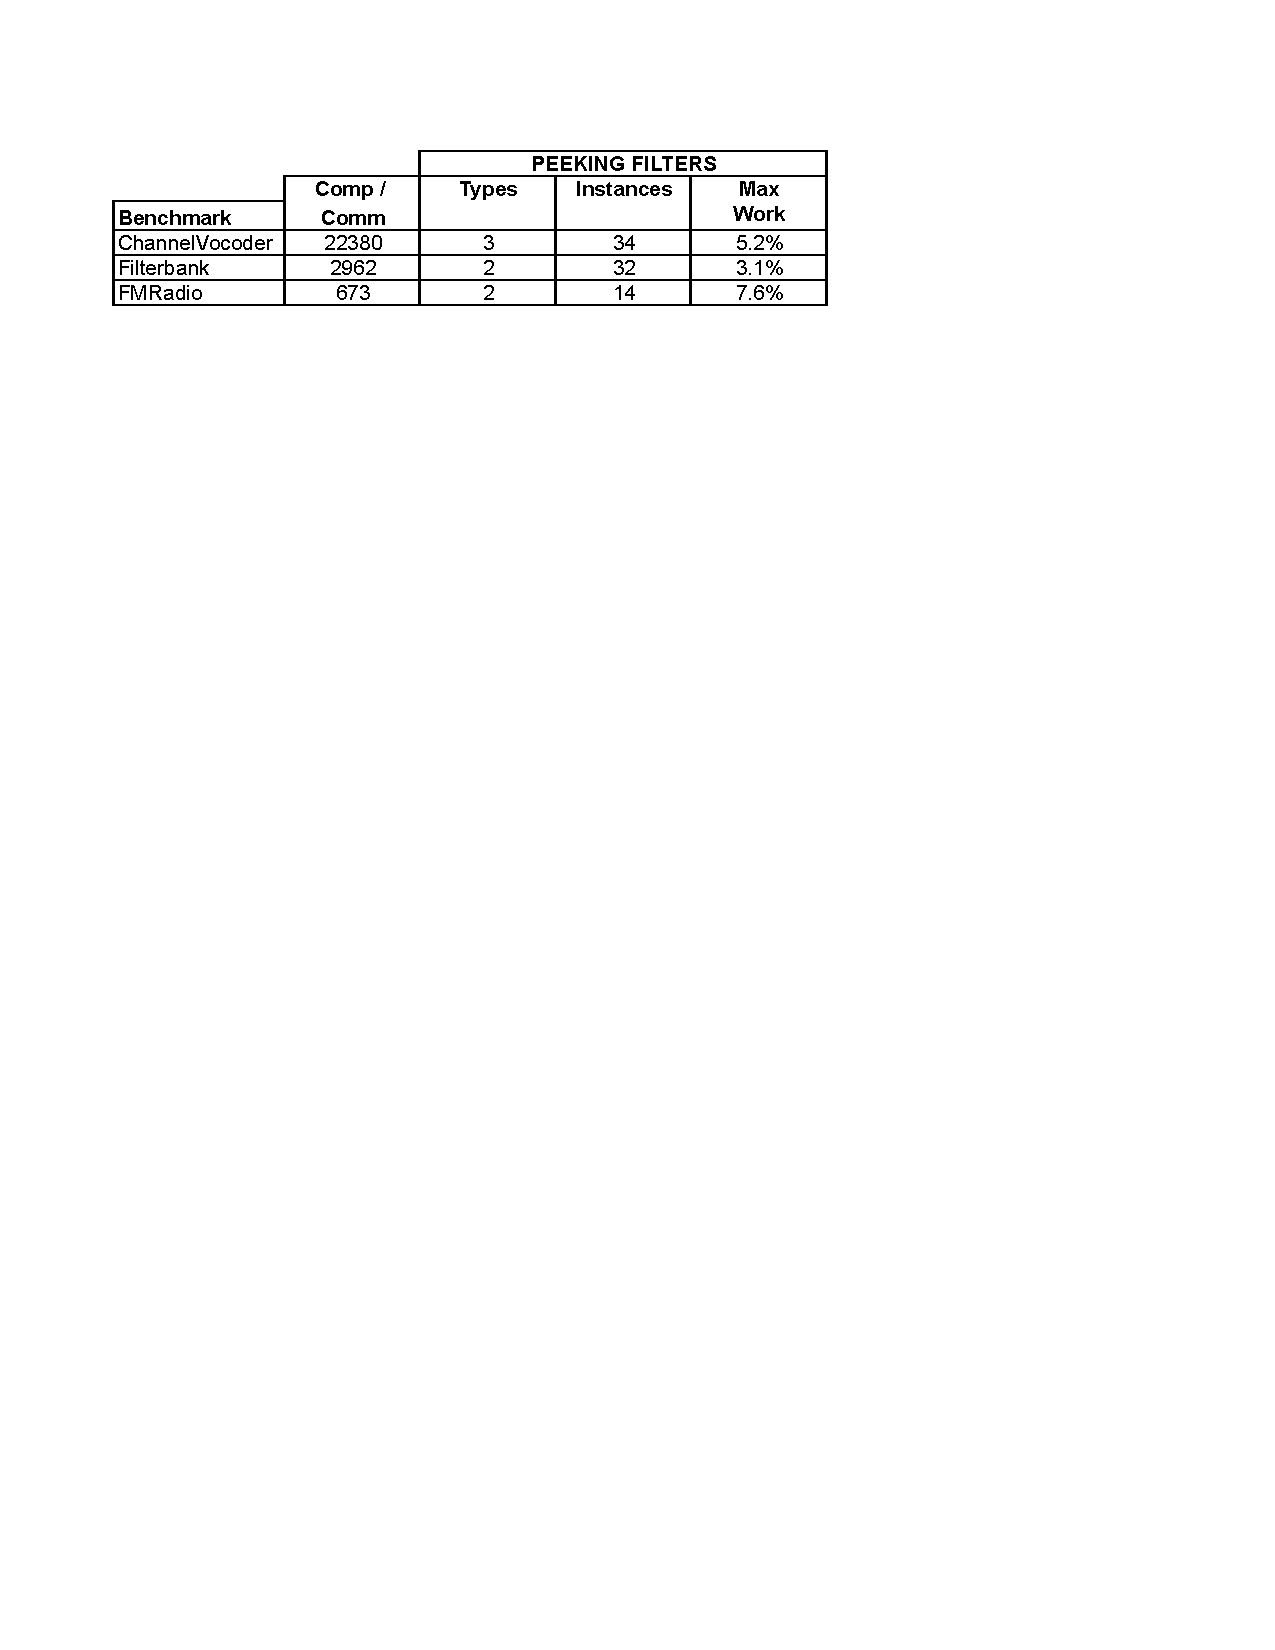
\includegraphics[width=3.3in]{figures/bench-char.pdf}}

\noindent ``Comp/Comm'' provides a static estimation of the
amount of computation to communication ratio by statically estimating the total
work of all the filters and dividing by the number items communicated
for the programmer-conceived graph's steady-state.  The remaining
statistics give the number of peeking filters types, number of peeking
filters instantiated at runtime, and a static estimation of the maximum
work in the single most loaded peeking filter.

We target 2 multicore architecture with different communication
mechanisms.  The Tilera Corporation's TILE64 Processor is a 64 core
system on a chip~\cite{tilera}.  Each core is an identical three-wide
VLIW. The code generated by the StreamIt
compiler for the TILE64 processor follows the remote store programming
(RSP) model~\cite{rsp10} in which each process has a private address
space, but each process can award remote processes write access to
their local memory. When a producer process has write access to a
consumer process's memory, the producer communicates directly with the
consumer via store instructions whose destination is an address in the
consumer's shared memory.  Communication is initiated by the producer,
and is fine-grained.  The consumer reads directly from it's local
memory (L2) when accessing input.

Our symmetric multiprocessor target is a 16-core architecture that is
comprised of four Intel Xeon E7350 multicore processors.  Each processor
is a 64-bit, quad-core with two dual-core dies.  Each die contains a 4
MB L2 cache shared across the two cores.  The front-side bus is clocked
at 1066 MHz.  We utilize the cache coherency mechanism of the
architecture for communication between cores. 

Through empirical experimentation on FMRadio, Filterbank, and
ChannelVocoder, we have settled on $T_{\mt{sharing}} =.10$ and
$T_{\mt{apply}} = 0.05$. These constants are the sweet stop for the two
architectures employed in the experimentation, being a good compromise
between buffer size and inter-core communication.

% \begin{figure*}[t]
% \centering
% \subfigure[]{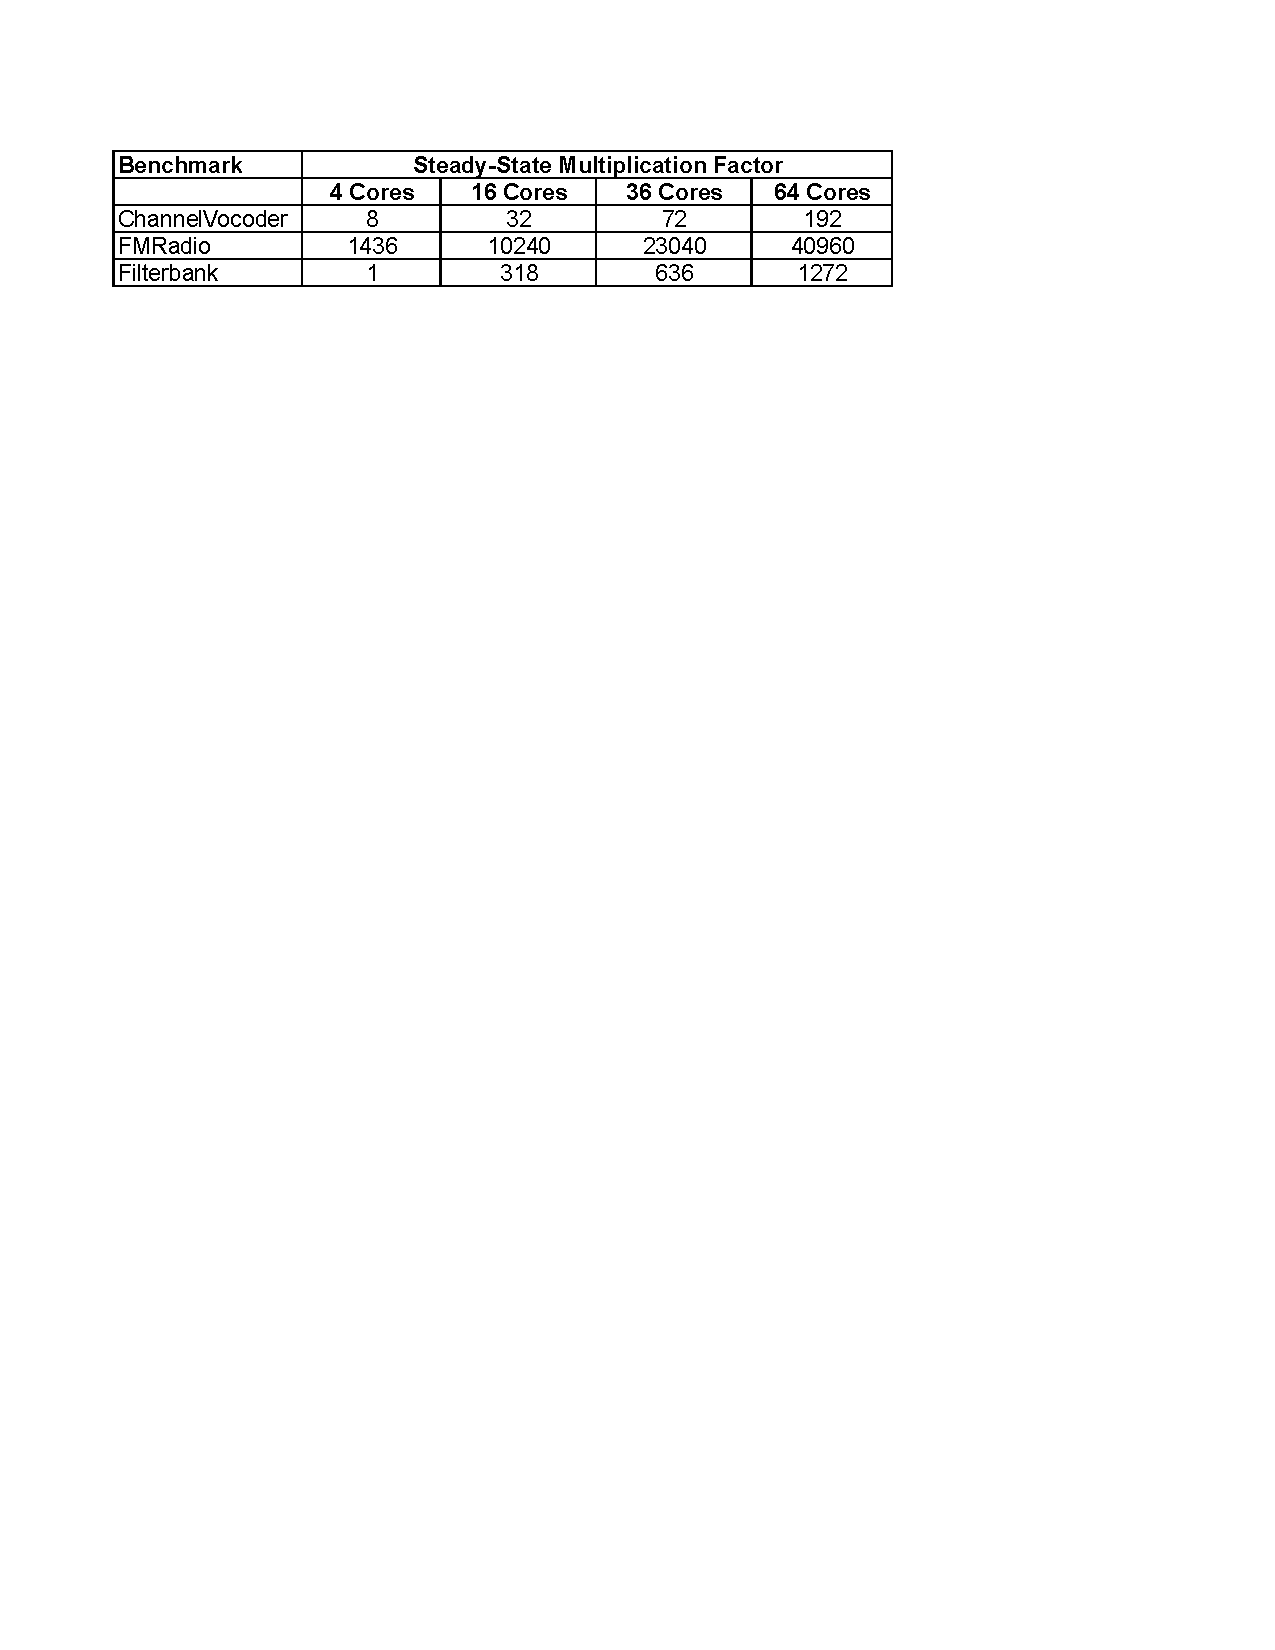
\includegraphics[width=3.7in]{figures/mult-table.pdf}} \\
% \subfigure[]{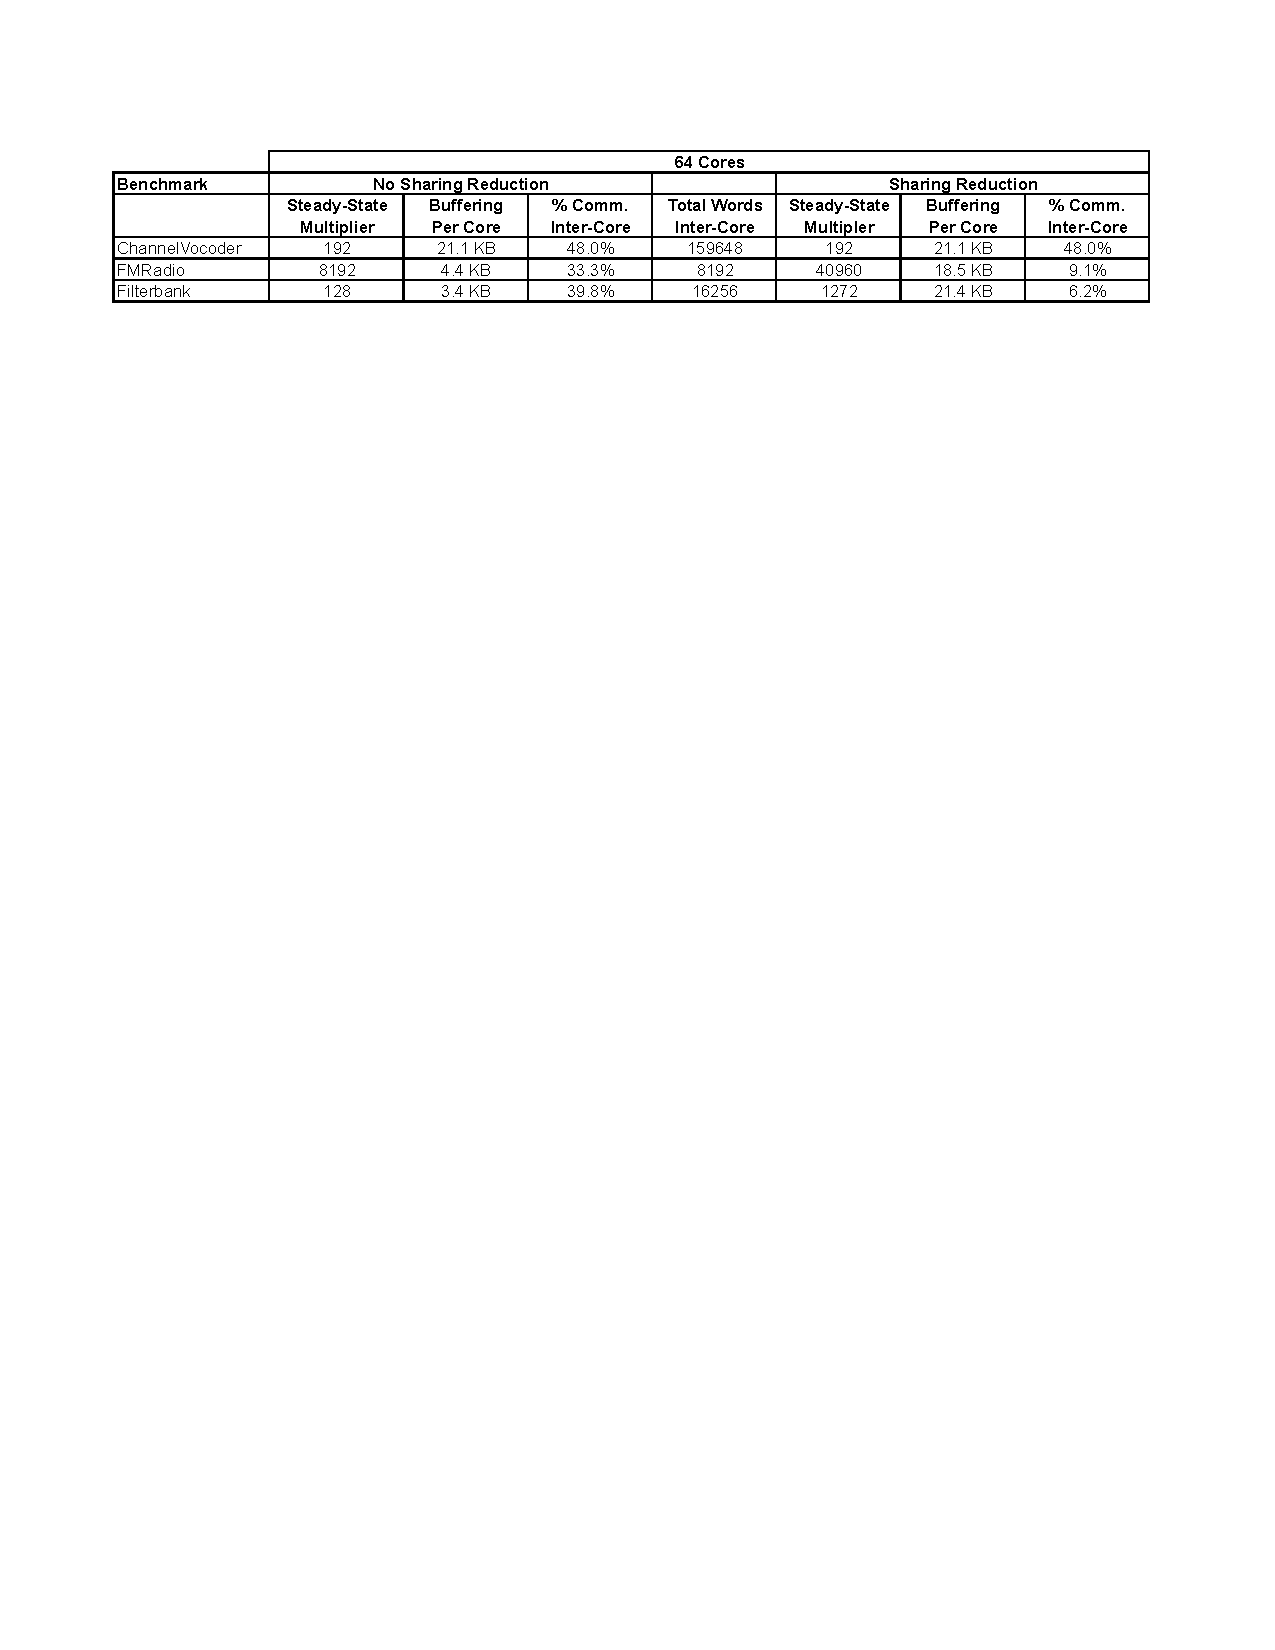
\includegraphics[width=6in]{figures/64-core-table.pdf}}
% \caption[Communication, multiplier and buffering statistics for
% benchmarks.]{
% Communication, multiplier and buffering characteristics for
% benchmarks: (a) gives the steady-state multipliers calculated for
% sharing reduction, (b) compares the steady-state with and without
% sharing reduction. 
% \label{fig:fission-table}}
% \end{figure*}

\begin{figure*}[t]
\centering
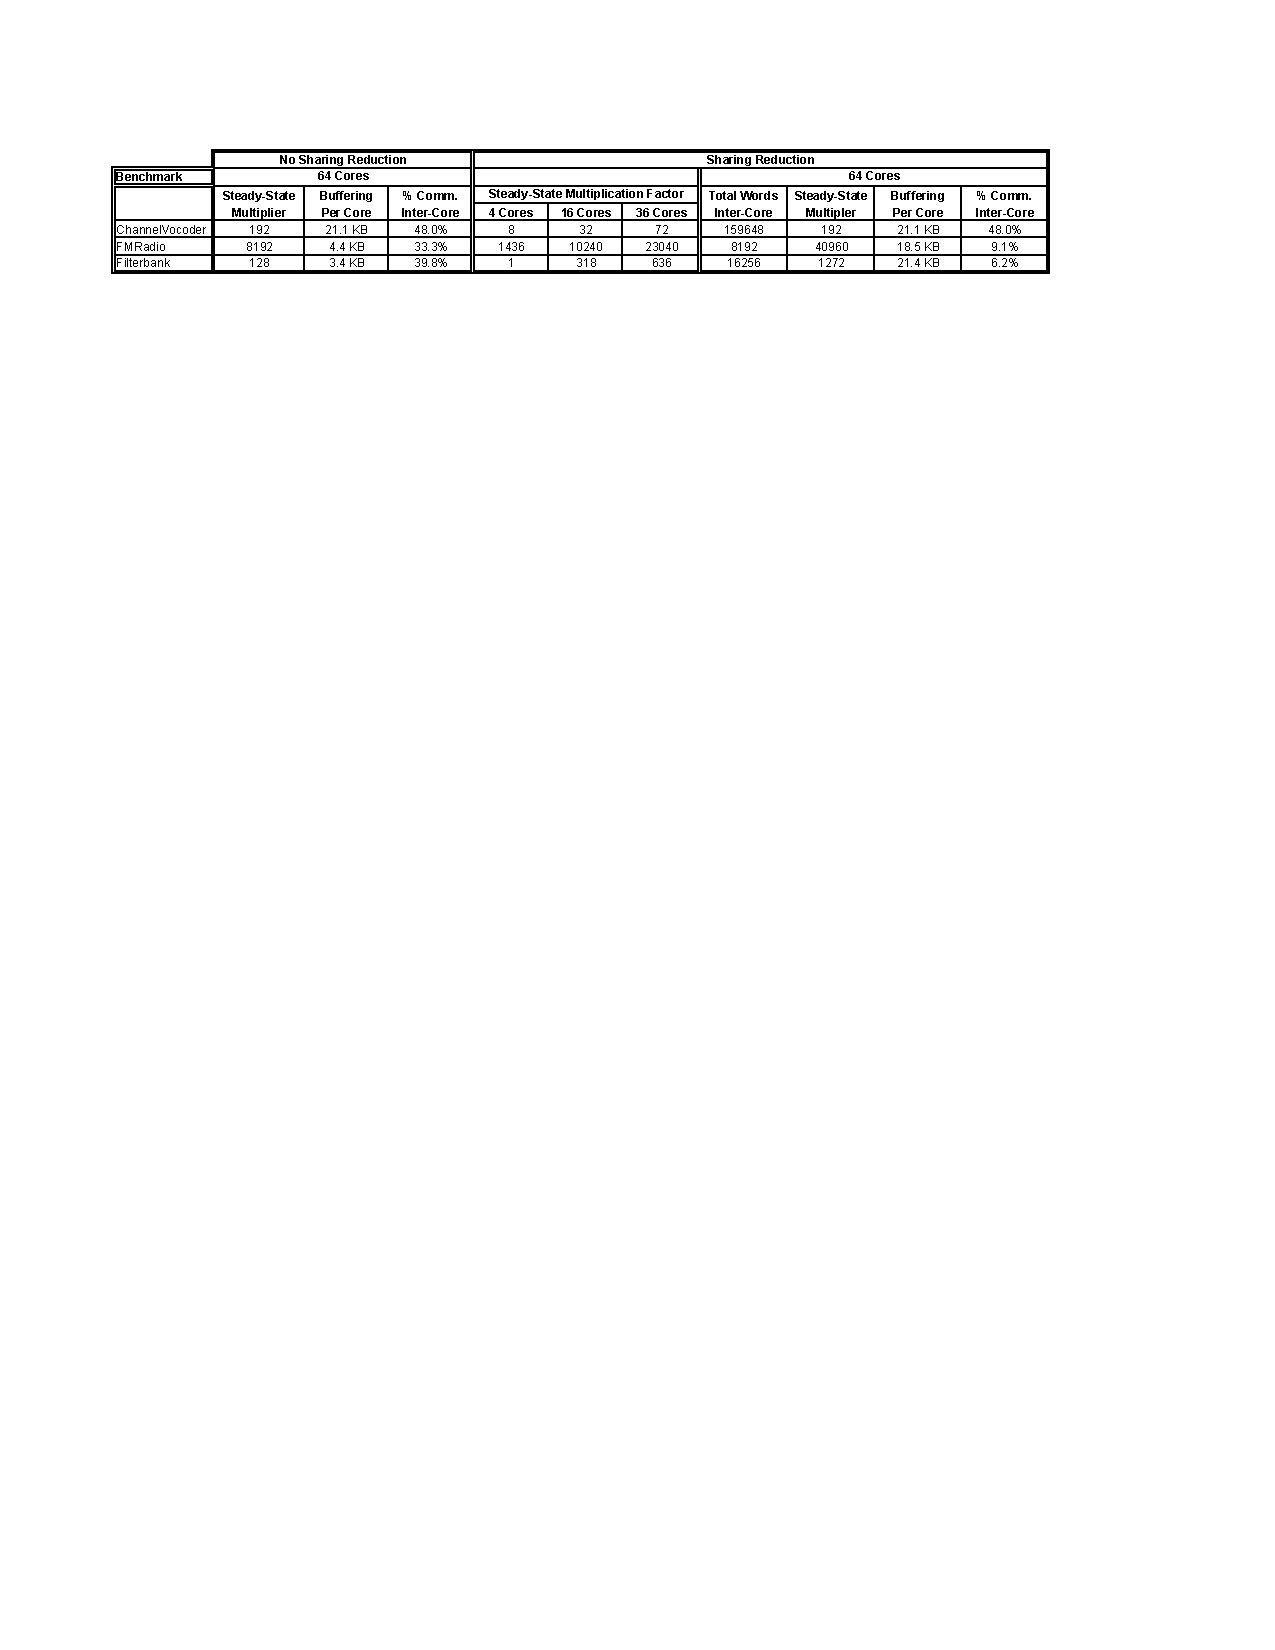
\includegraphics[width=6.1in]{figures/big-table.pdf}
\caption{\label{fig:big-table}  Steady-state multiplicity, buffering,
  and communication for fission with and without sharing reduction.}
\end{figure*}

% \begin{figure}[t]
% \centering
% 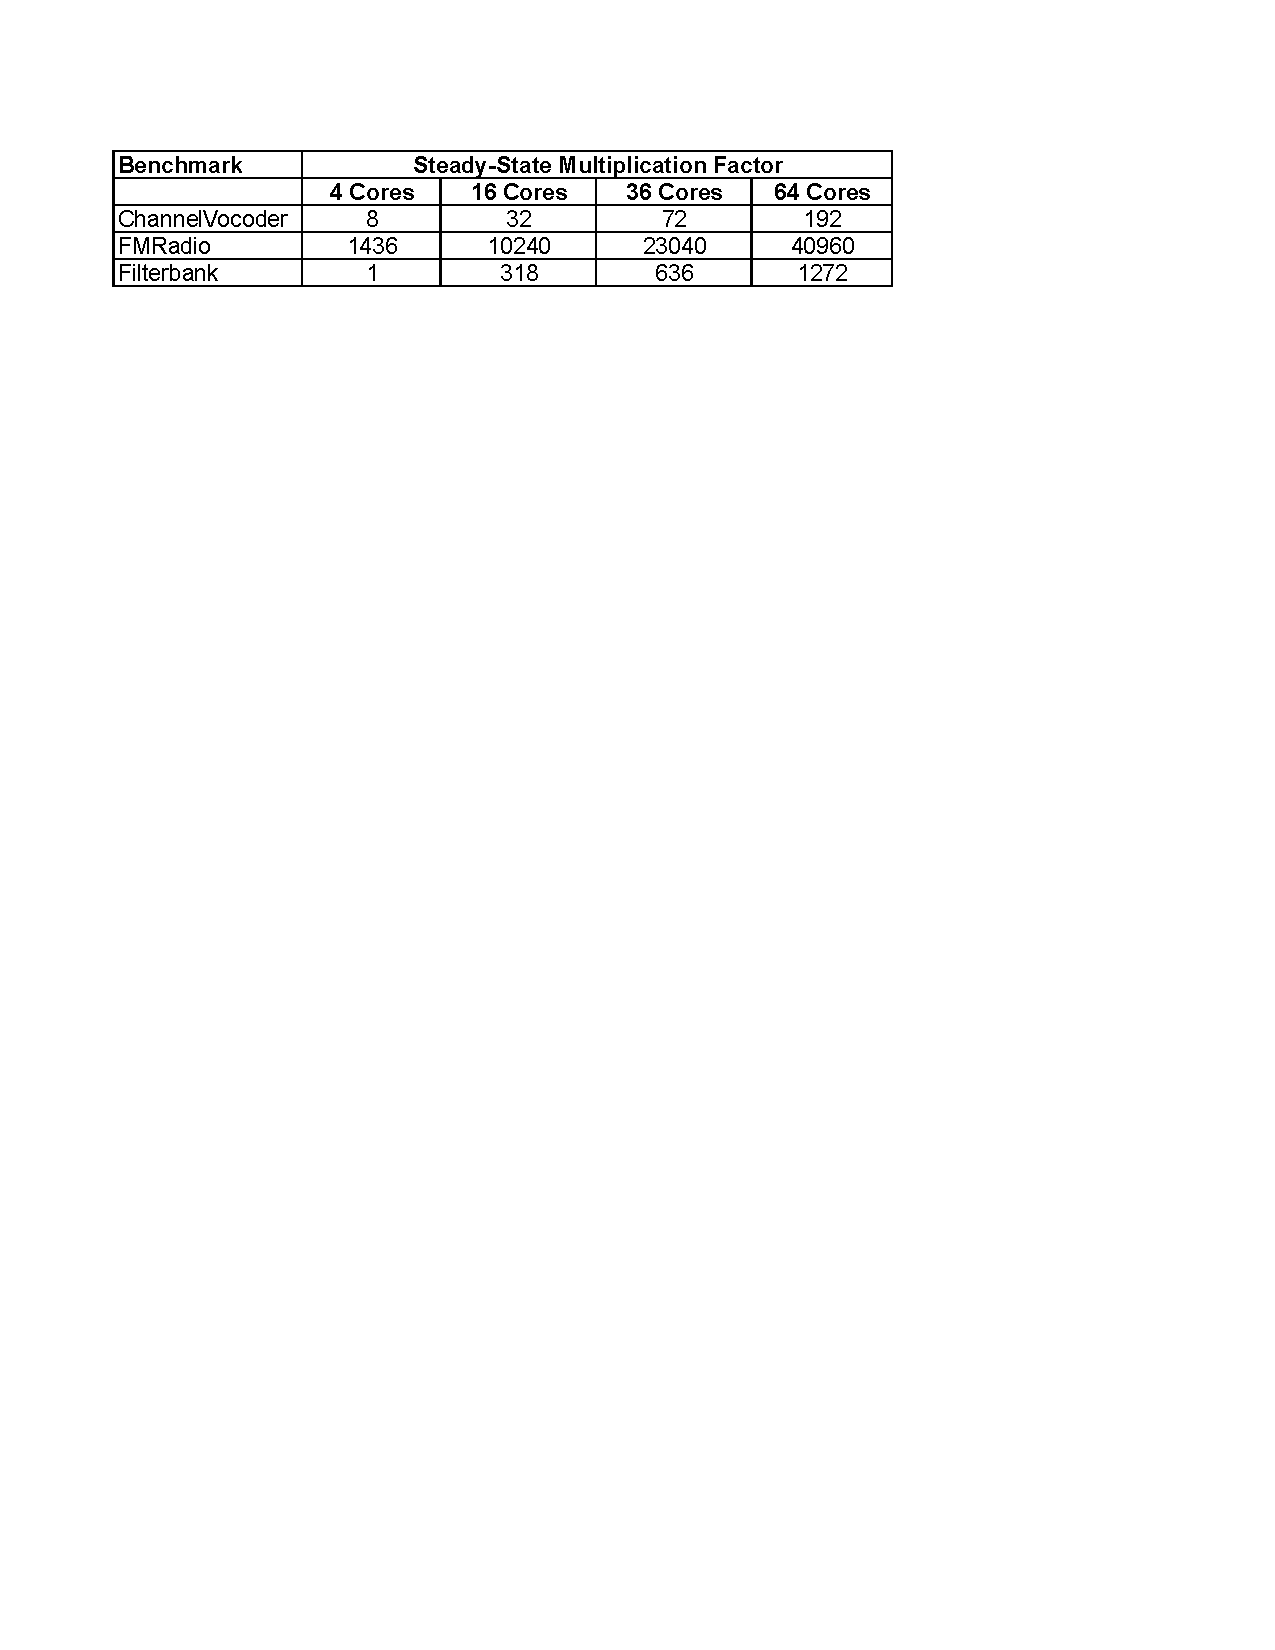
\includegraphics[width=3.3in]{figures/mult-table.pdf}
% \caption{\label{fig:mult-table}  The steady-state multipliers calculated for
% sharing reduction.}
% \end{figure}

% \begin{figure*}[t]
% \centering
% 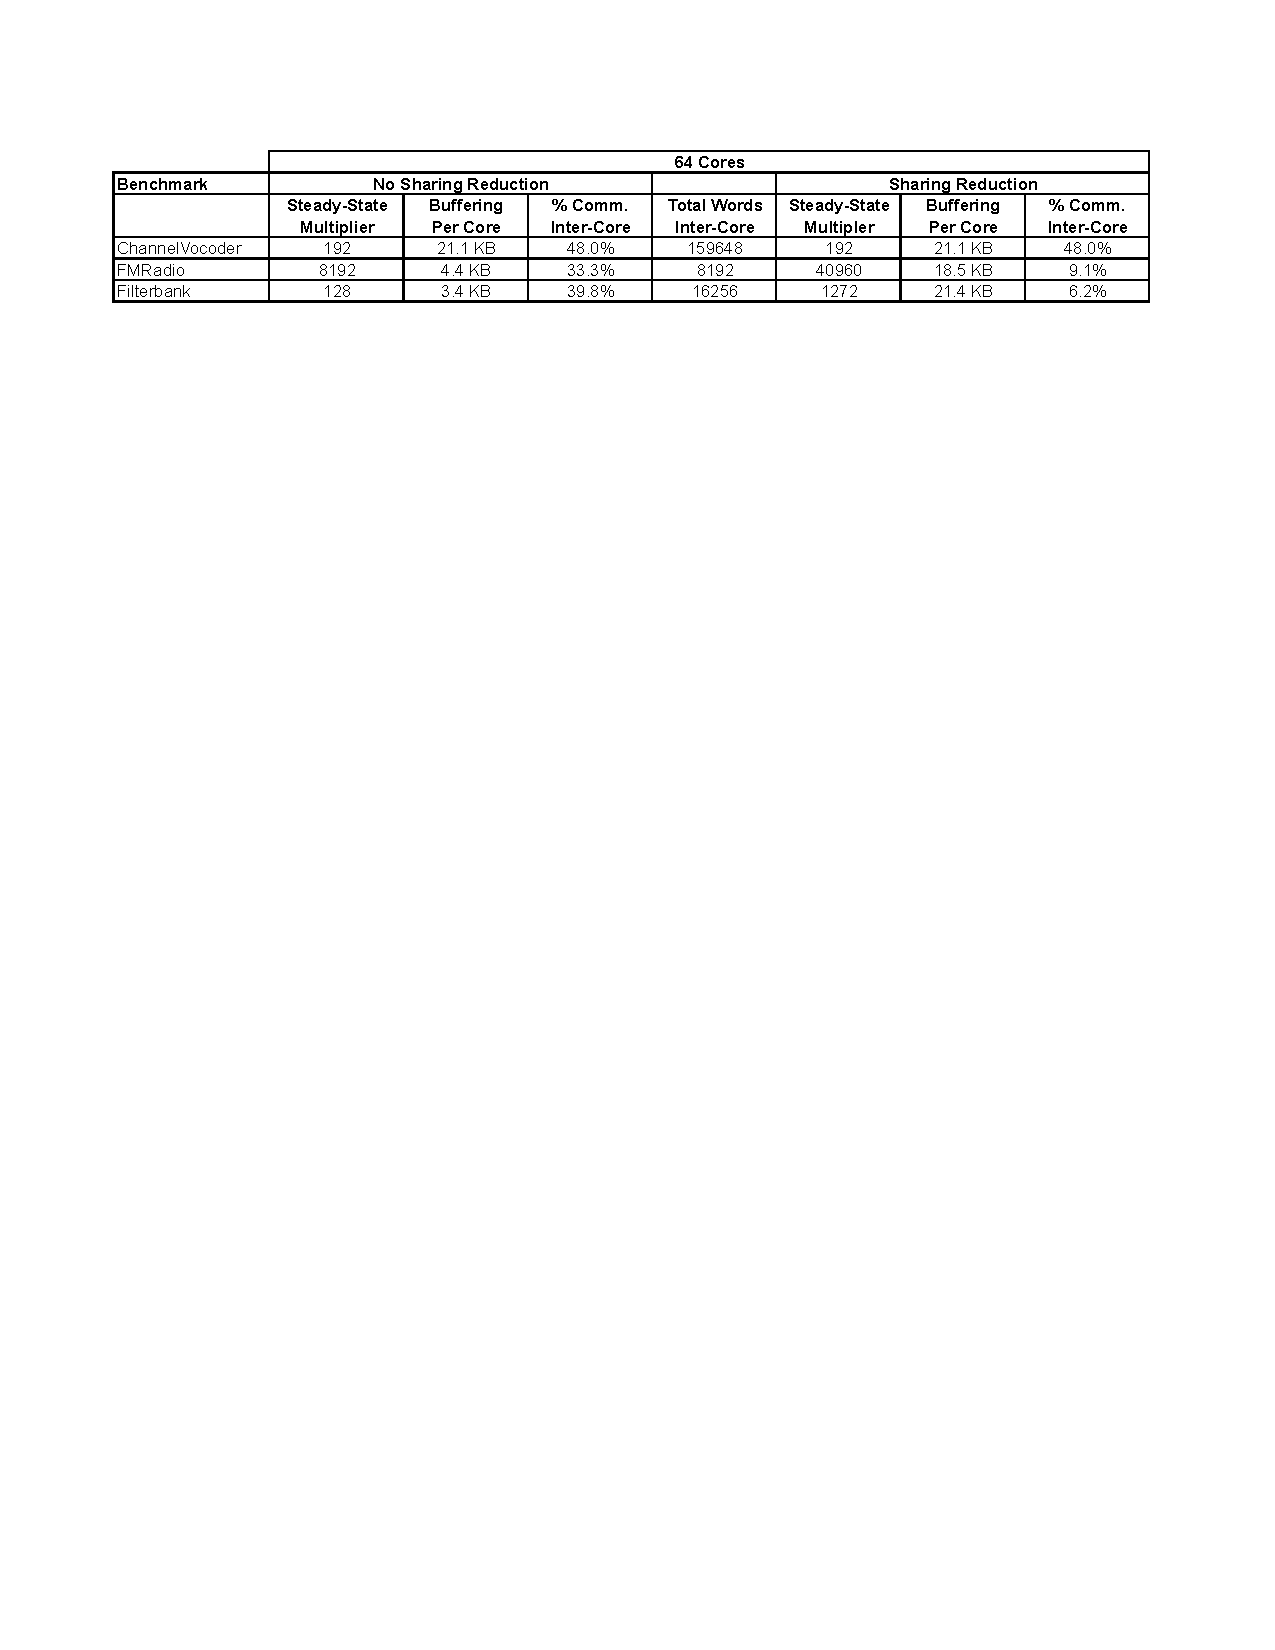
\includegraphics[width=6in]{figures/64-core-table.pdf}
% \caption{ Multiplier, buffering and communication for the steady-state with and without
% sharing reduction. 
% \label{fig:fission-table}}
% \end{figure*}

Figure~\ref{fig:big-table} compares the steady-state with and
without sharing reduction for a 64-core mapping, as well as gives the
constant $c$ calculated by sharing reduction for 4, 16, and 36.  The
factor is larger for FMRadio because one filter has $C(f) \gg o(S,
f)$.  The multiplication factor affects both latency and buffer sizes
adversely.  The application designer will have to decide if the
latency of these techniques can be borne given the application
criteria.  The total buffering requirement is increased when the
steady-state is increased.  However, since we are then fissing, the
buffer is divided amongst the fission products, and the {\it per-core}
buffering requirement is unaffected by the increase.  For example,
FMRadio, has a per-core 18 KB buffering requirement across all
configurations (4, 16, 36, and 64 cores).  This requirement fits in
the per-core L2 size of 64 KB for the Tile64.

 For ChannelVocoder,
sharing reduction has no effect because most of the peeking filters do
not satisfy $T_{\mt{apply}} = 0.05$ because of differing fission
factors between producers and consumers.  For the peeking filters that do,
the steady-state multiplier required for legal general fission for the
graph is enough to assure $T_{\mt{sharing}}$ is met.  Even though
sharing reduction has no effect for ChannelVocoder, general fission
avoids the 38\% of total items that were unnecessary duplicated by
DupDec.

For FMRadio and Filterbank, sharing reduction leads to significant
decreases in the percentage of total items communicated inter-core for
each steady-state.  The buffer requirement is increased an average of
5.2x for these benchmarks.  The total number of words communicated
inter-core during each steady-state is the same, with and without
sharing reduction.  However, the steady-state is greater in the
sharing reduction case, thus producing more outputs.

\begin{figure}[t]
\centering
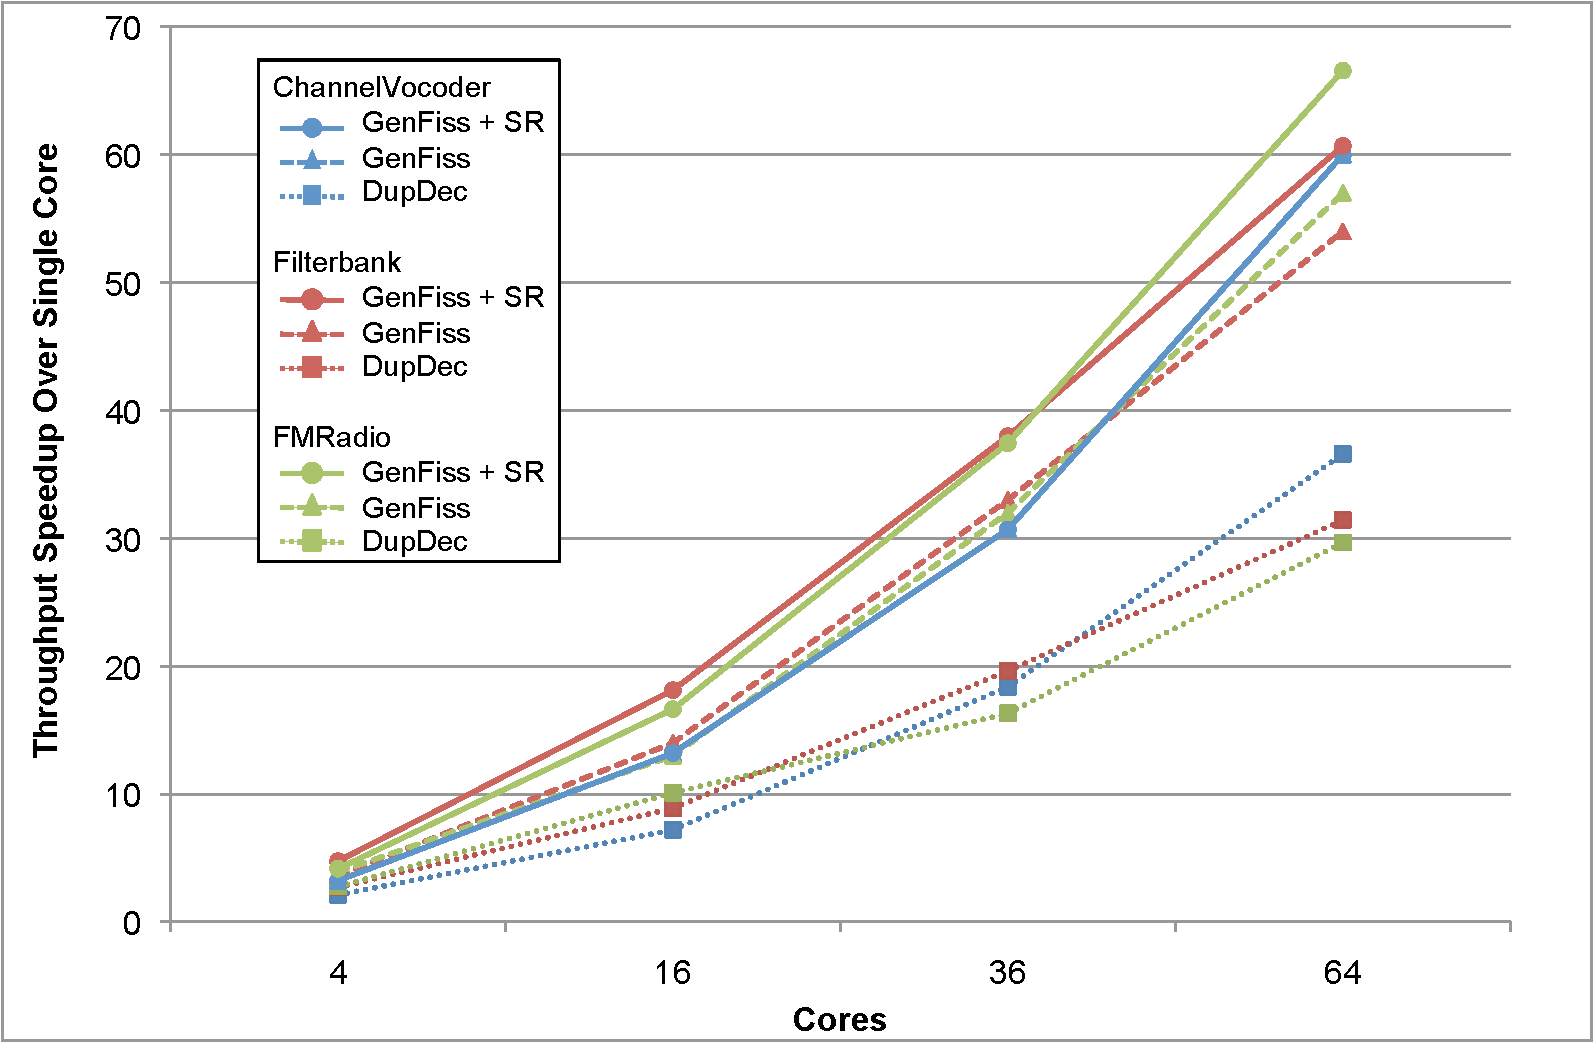
\includegraphics[width=3.3in]{figures/tilera-chart.pdf}
\caption[Comparing the fission techniques on the TILE64.]{
  Evaluation for DupDec versus general fission versus general fission with sharing reduction
  4, 16, 36, and 64 cores on the TILE64.  \label{fig:tilera-chart}}
\end{figure}

Figure~\ref{fig:tilera-chart} gives the performance results for the
Tilera TILE64 architecture.  We present results for DupDec, general
fission, and general fission with sharing reduction for 4, 16, 36, and
64 core configurations, with throughput normalized to single-core
throughput.  General fission with sharing reduction outperforms
DupDec by an average of 1.8x for the three benchmarks when targeting
64 cores. The average 64-core speedup over single core is 62.3x for the
general fission plus sharing reduction for these three benchmarks.

FMRadio experiences the most significant gain from general fission
plus sharing reduction over DupDec (67x versus 30x, respectively, for
64 cores).  FMRadio has the lowest computation to communication ratio
of the 3 benchmarks.  Furthermore, each filter of is fissed by the
number of cores targeted.  For 64 cores, each filter is fissed 64
ways.  DupDec must perform a global all-to-all communication involving
all 64 cores between each level of the graph!
 
ChannelVocoder achieves a 60x speedup for general fission over a
single core.  This is not perfectly linear because of the parallel
mapping; asymmetries exist between the extent of task parallelism and
the number of cores (see~\ref{mgordon-asplos06}).  The speedup over
DupDec (1.62x) is more modest because the width of many of the
fission applications is 3, so DupDec is duplicating input data to
groups of 3 filters.  Filterbank is similar, the width of fission is 4
for all filters when targeting 64 cores.

Sharing reduction is required to achieve scalable speedups for both
FMRadio and Filterbank.  For FMRadio, sharing reductions leads to a
17\% speedup increase for 64 cores.  This because sharing reduction
significantly reduces the number of remote write store instructions
required per output.  This affects FMRadio because of its low
computation to communication ratio.  Sharing reduction sees a 12\%
increase on Filterbank, as Filterbank has a larger computation to
communication ratio.

\begin{figure}[t]
\centering
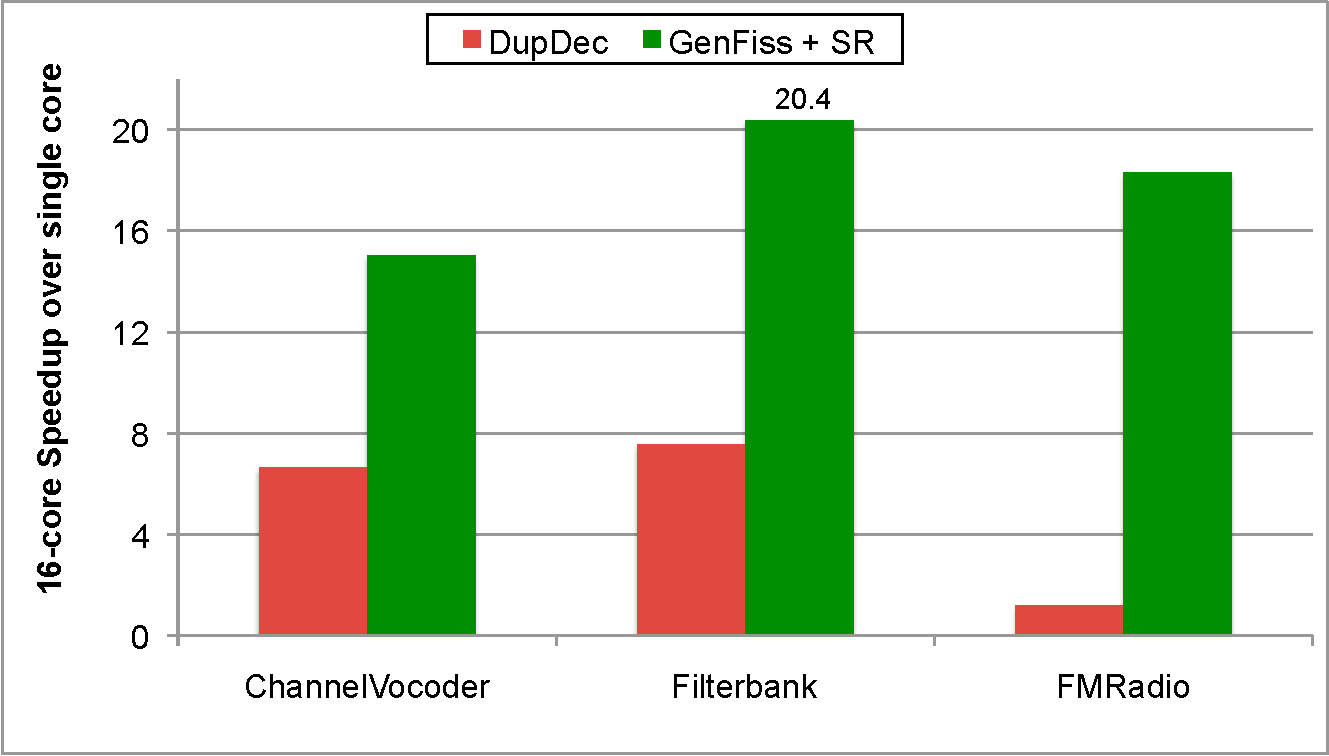
\includegraphics[width=3.3in]{figures/smp-chart.pdf}
\caption[Comparing the fission techniques on the 16-core SMP.]{
  Evaluation for DupDec versus general fission with sharing reduction
  for the 16-core SMP architecture.  \label{fig:smp-chart}}
\end{figure}

Our techniques enable scalable parallelization, with a mean speedup of
17x for our 3 benchmarks on the SMP.  Figure~\ref{fig:smp-chart} gives
the 16-core speedup comparison for DupDec versus general fission with
sharing reduction for our target SMP architecture.  The mean speedup
increase for general fission with sharing reduction over DupDec is
6.7x.  FMRadio again sees the largest speedup increase in the
comparison at 13.0x.  The reasons for this large speedup are similar
as given in the previous section.  However, the SMP communication
mechanism is not as efficient as the TILE64, thus general fission with
sharing reduction gives a greater speedup because reducing inter-core
communication has more impact.

\section{Related Work}
\label{sec:related}

% BILL

%Signal~\cite{Signal}, 
%Lucid~\cite{Lucid77}, and
%Occam~\cite{Occam}, and Sisal \cite{sisal}.
%Parallel Haskell~\cite{ph}
In addition to StreamIt, there are a number of stream-oriented
languages drawing from domains such as functional, dataflow, CSP and
synchronous programming~\cite{survey97}.  The Brook language is
architecture-independent and focusses on data
parallelism~\cite{brook04}.  Stream kernels are required to be
stateless, though there is special support for reducing streams to a
single value.  Stream\-C/Ker\-nel\-C is lower level than Brook;
kernels written in KernelC are stiched together in StreamC and mapped
to the data-parallel Imagine processor~\cite{imagine03ieee}.  SPUR
adopts a similar decomposition between ``microcode'' stream kernels
and skeleton programs to expose data parallelism~\cite{spur05samos}.
Cg exploits pipeline parallelism and data parallelism, though the
programmer must write algorithms to exactly match the two pipeline
stages of a graphics processor~\cite{cg03}.  Compared to these
languages, StreamIt places more emphasis on exposing task and pipeline
parallelism (all the languages expose data parallelim).
%and on sliding window operations (filters that peek).  
By adopting the synchronous dataflow model of execution~\cite{lee87},
StreamIt focusses on well-structured programs that can be aggressively
optimized.  The implicit infinite loop around programs is also a key
StreamIt characteristic that enables the transformations in this
paper.  Spidle is also a recent stream language that was influenced by
StreamIt~\cite{spidle03}.
%and Lucid Synchrone~\cite{Lucid-Synchrone}.
%Synchronous languages which
%target embedded applications include Esterel~\cite{Esterel},
%Lustre~\cite{Lustre}, and Additional

Liao et al. map Brook to multicore processors by leveraging the affine
partitioning model~\cite{liao06brook}.  While affine partitioning is a
powerful model for parameterized loop-based programs, in StreamIt we
simplify the problem by fully resolving the program structure at
compile time.  This allows us to schedule a single steady state using
flexible, non-affine techniques (e.g., simulated annealing) and to
repeat the found schedule for an indefinite period at runtime.
Gummaraju and Rosenblum map stream programs to a general-purpose
hyperthreaded processor~\cite{gummaraju05micro}.  Such techniques
could be integrated with our spatial partitioning to optimize per-core
performance.  Gu et al. expose data and pipeline parallelism in a
Java-like language and use a compiler analysis to efficiently extract
coarse-grained filter boundaries~\cite{du03sc}.  Ottoni et al. also
extract decoupled threads from sequential code, using hardware-based
software pipelining to distribute the resulting threads across
cores~\cite{ottoni05decoupled}.  By embedding pipeline-parallel
filters in the programming model, we focus on the mapping step.

%%%%%%%%%%%%%%%%%%%%%%%%%%%%%%%%%%%%%%%%%%%%%%%%%%%%%%%%%%%%%%%%%%%%%

Previous work in scheduling computation graphs to parallel targets has
focused on partitioning and scheduling techniques that exploit task
and pipeline parallelism~\cite{SDFSched, SDFSched2,may87communicating,
DAGSched, pipeline-sdf}.  Application of loop-conscious
transformations to coarse-grained dataflow graphs has been
investigated.  Unrolling (or ``unfolding'' in this domain) is employed
for synchronous dataflow (SDF) graphs to reduce the initiation
interval but they do not evaluate mappings to actual
architectures~\cite{unfolding,unfolding2}. Software pipelining
techniques have been applied to SDF graphs onto various embedded and
DSP targets~\cite{bakshi99,chatha-02}, but has required programmer
knowledge of both the application and the architecture. To our
knowledge, none of these systems automatically exploit the combination
of task, data, and pipeline parallelism.  Furthermore, these systems
do not provide a robust end-to-end path for application
parallelization from a high-level, portable programming language.

%% Previous work on instruction-level software pipelining has focused
%% mostly on scheduling machine instructions in a loop via modulo
%% scheduling~\cite{rau81,lam-softpipe}.  The algorithms devised must
%% account for tight resource constraints and complex instruction
%% dependences. Our software-pipelining problem is much less constrained,
%% enabling us to employ a simple greedy heuristic.  

%% Furthermore, a traditional modulo scheduling algorithm is not needed
%% because we have an implicit loop barrier at the end of each
%% steady-state.  ILP compilers for clustered VLIW
%% architectures~\cite{Bulldog,Multiflow,lee98spacetime,qian02} must
%% partition instructions and assign them to clusters as part of the
%% instruction scheduling. Clustering is analogous to our application of
%% filter fusion in our software pipelining algorithm.

\section{Conclusion}
\label{sec:conclusion}

In this paper, we describe the StreamIt compiler for the Raw
architecture.  The stream graph of a StreamIt program exposes the data
communication pattern to the compiler while the lack of global
synchronization frees the compiler to radically reoganize the program
for efficient execution on the underline architecture. The StreamIt
compiler demonstrates the power of this flexibility by totally
reoganizing large programs for better load balance. We were able to
map many of programs on to the Raw processor and obtain good
performance.

We introduce a collection of optimizations, vertical and horizontal
filter fusion, vertical and horizontal filter fission and filter
reordering transformations, that can be used to restructure stream
graphs.  We show that by applying these transformations we can map a
high-level stream program, written to reflect the composition of the
application, onto Raw and achieve good processor utilization and load
balance, leading to a factor of three speedup on two applications.

Unlike all previous streaming languages, the structured streams of
StreamIt makes it possible for us to approach the optimization and
parallelization problems in a very systermatic manner. It enables us
to define multiple optimizations -- targetting different constructs
and requirements -- and to compose them them in a hirearchical manner.

The ability to do global transformations across multiple filters, that
may have originated from very different parts of the application,
makes it possible for the compiler to find optimization opportunities
that may ellude even an experience programmer.  Such capabilities
enables the programmers to write protable streaming applications and
map them efficiently onto any given architecture. This has the
potential of creating a programming standard for emerging
communication exposed architectures.  The StreamIt compiler takes a
fist step towards this goal.



{\scriptsize
{\bibliographystyle{abbrv}
\bibliography{references}
}
}
\end{document}
